\documentclass[12pt,onecolumn,a4paper]{article}
\usepackage{epsfig,graphicx,subfigure,amsthm,amsmath}
\usepackage{color,xcolor}     
\usepackage{xepersian}
\usepackage{cite}
\usepackage{fontspec}
\usepackage{multirow}

\settextfont[Scale=1]{BMitra}
\setlatintextfont[Scale=0.8]{Vazir-Regular}


\begin{document}
\title{گزارش تکلیف 4 درس یادگیری ماشین} 
\author{کسرا سینایی\\
شماره دانشجویی ۸۱۰۶۹۶۲۵۴\\
}
\date{\today}
\maketitle
\thispagestyle{empty}
\newpage
\section{سوال یک}
\subsection*{الف}
در روش \lr{KNN} هرچه مقدار $K$ را کوچکتر انتخاب کنیم پیچیدگی مدل و مرز تصمیم افزایش می‌یابد و به همین نسبت جنرالیزیشن مدل کمتر و حساسیت به نویز نیز بیشتر می‌شود. در واقع هر چه $K$ کوچکتر باشد واریانس بیشتر خواهد بود. با افزایش $K$ به حد بهینه‌ای برای مدل می‌رسیم و افزایش بیشتر آن منجر به خطای بایاس می‌شود.
\\
در تخمین پنجره پارزن هایپرپارامتر مدل طول پنجره در تابع کرنل می‌باشد. این پارامتر ($h_{n}$) مانند یک \lr{smoothing factor} عمل می‌کند. هر چه طول پنجره بزرگتر باشد شکل تابع به دست آمده برای توزیع متغییرها نرم‌تر می‌شود. برای $h$ های بسیار کوچک تخمین نان‌پارامتری پارزن به تابع دلتا دیراک شبیه خواهد شد. به زبان دیگر انتخاب طول بزرگ برای پنجره منجر به خطای بایاس و انتخاب اندازه کوچک برای طول پنجره منجر به خطای واریانس می‌شود.
\subsection*{ب}
در روش‌های پارامتریک فرض می‌کنیم داده‌ها از یک توزیع شناخته شده و فرمول‌بندی شده مانند گوسی، پواسون و ... آمده‌اند و برای توصیف آن‌ها به تخمین پارامترهای مدل فرض شده می‌پردازیم.
\\
در روش‌های نان‌پارامتری هیچ فرض اضافه‌ای برای مدل حاکم بر داده‌های یادگیری قرار نمی‌دهیم و با قوانینی مانند نزدیک‌ترین همسایه‌، استفاده از تابع کرنل و ... توزیعی دلخواه به داده‌های یادگیری فیت می‌کنیم.
\subsection*{ج}
چون این روش‌ها نان‌پارامتریک هستند لازم است برای پیش‌بینی نقاط دیده نشده تمام مجموعه یادگیری را همراه با مدل نگه داریم. (در واقع مدل مستق و به کمک یک تابع و چند پارامتر تعریف نشده که بتوان با استفاده از آن پیش بینی کرد، بلکه مدل با استفاده از داده‌های مجموعه یادگیری در هر نقطه تعریف می‌شود)
\\
با افزایش ابعاد فیچرها برای دست‌یابی به تخمینی دقیق تعداد نقاط مورد نیاز در دیتاست به صورت نمایی افزایش می‌یابد و در مواردی که نتوانیم حجم داده‌ها را افزایش دهیم ممکن است دچار نفرین ابعادی شویم.

\subsection*{د}
در روش پنجره پارزن مفهوم حجم وابسته به کرنل استفاده شده است. برخی کرنل‌ها به تمامی نقاط موجود در دیتاست وزن می‌دهند (مانند کرنل گوسی) و برخی کرنل‌ها مانند \lr{hyper cube kernel} تنها داده‌های موجود در ابر مکعب حول نقطه مورد نظر را برای طبقه بندی یا تخمین احتمال در نظر می‌گیرند.
\\
در روش \lr{KNN} حجم با یک ابر کره که شعاع آن فاصله دورترین نقطه در بین \lr{K} همسایه نقطه‌ای که می‌خواهیم احتمال آن را به دست بیاوریم، تعریف می‌شود.

\newpage
\section{سوال دو}
در این سوال می‌خواهیم نشان دهیم که سلول‌های \lr{voronoi} تشکیل شده با الگوریتم نزدیک‌ترین همسایه محدب هستند. \\
به ازای هر دو نقطه درون یک سلول، خط وصل کننده آن‌ها نیز داخل سلول قرار خواهد گرفت ،فرض کنید $x^{*}$ در یک سلول با لیبلی مشخص واقع شده باشد و $y$ نیز نقطه‌ای با یک لیبل متفاوت از $x^{*}$ باشد. در این حالت ابر صفحه‌ای وجود دارد که فضا را طوری تقسیم می‌کند که یک طرف آن نقاط به $x^{*}$ نزدیک تر هستند و طرف دیگر آن نقاط به $y$ نزدیک ترند. اگر نقاط $x(0)$ و $x(1)$ در سلول متعلق به $x^{*}$ قرار داشته باشند خطی که این دو نقطه را به هم وصل می‌کند نیز به صورت: $x(\lambda) = (1 - \lambda)x(0) + \lambda x(1); 0 \leq \lambda \leq 1$ خواهد بود. این خط نیز به طور کامل درون سلول متعلق به نقطه $x^{*}$ قرار خواهد گرفت.
چون فضای نصف شده توسط ابر صفحه محدب است، تمامی نقاط موجود بر روی خط تعریف شده ($x(\lambda)$) نیز به به $x^{*}$ نزدیک تر هستند تا $y$. \\
این موضوع به ازای تمام نقاط موجود در \lr{Voronoi Cell} متعلق به نقطه $x^{*}$ صادق است. همچنین برای سایر سمپل‌ها نیز صادق است (شرطی برای $y$ نداریم) بنابراین \lr{Voronoi Cell} تشکیل شده با قانون نزدیک ترین همسایه همواره محدب می‌باشند.
\newpage
\section{سوال سه}
\subsection*{الف}
\begin{figure}[h!]
    \begin{center}
    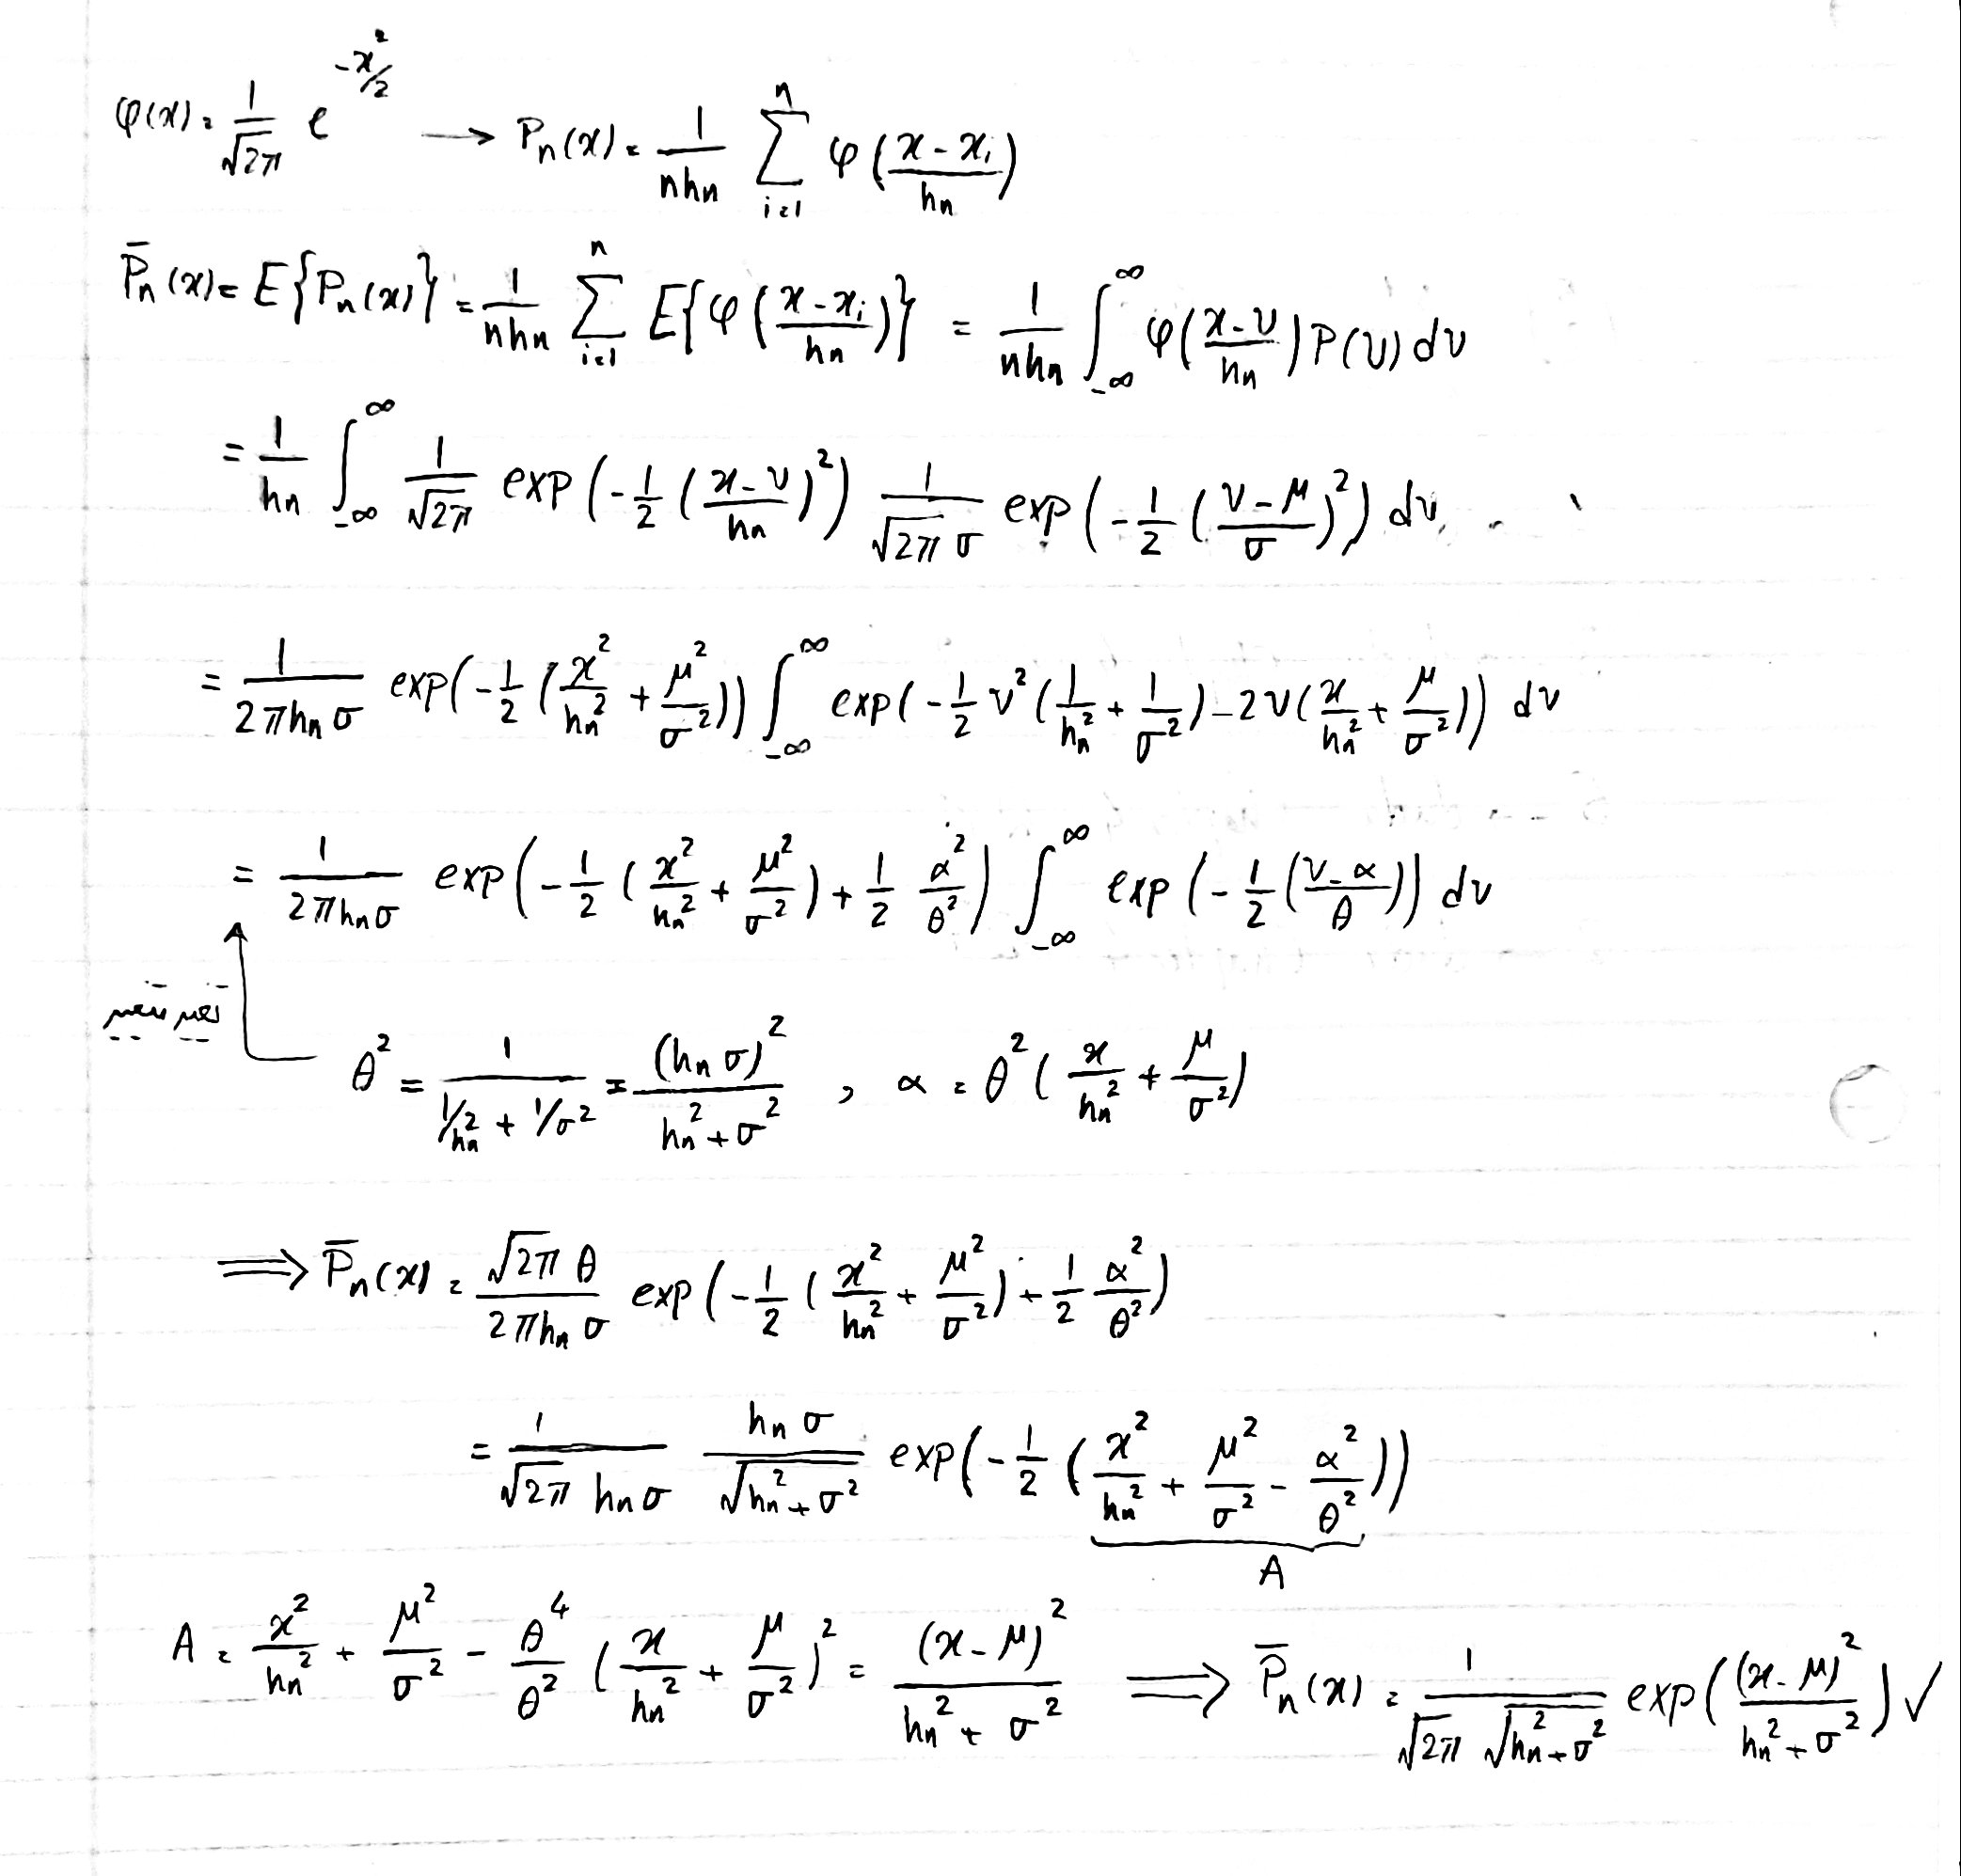
\includegraphics[width=\linewidth]{hand_written/31.jpg}
    \end{center}
\end{figure}
\newpage

\subsection*{ب}
\begin{figure}[h!]
    \begin{center}
    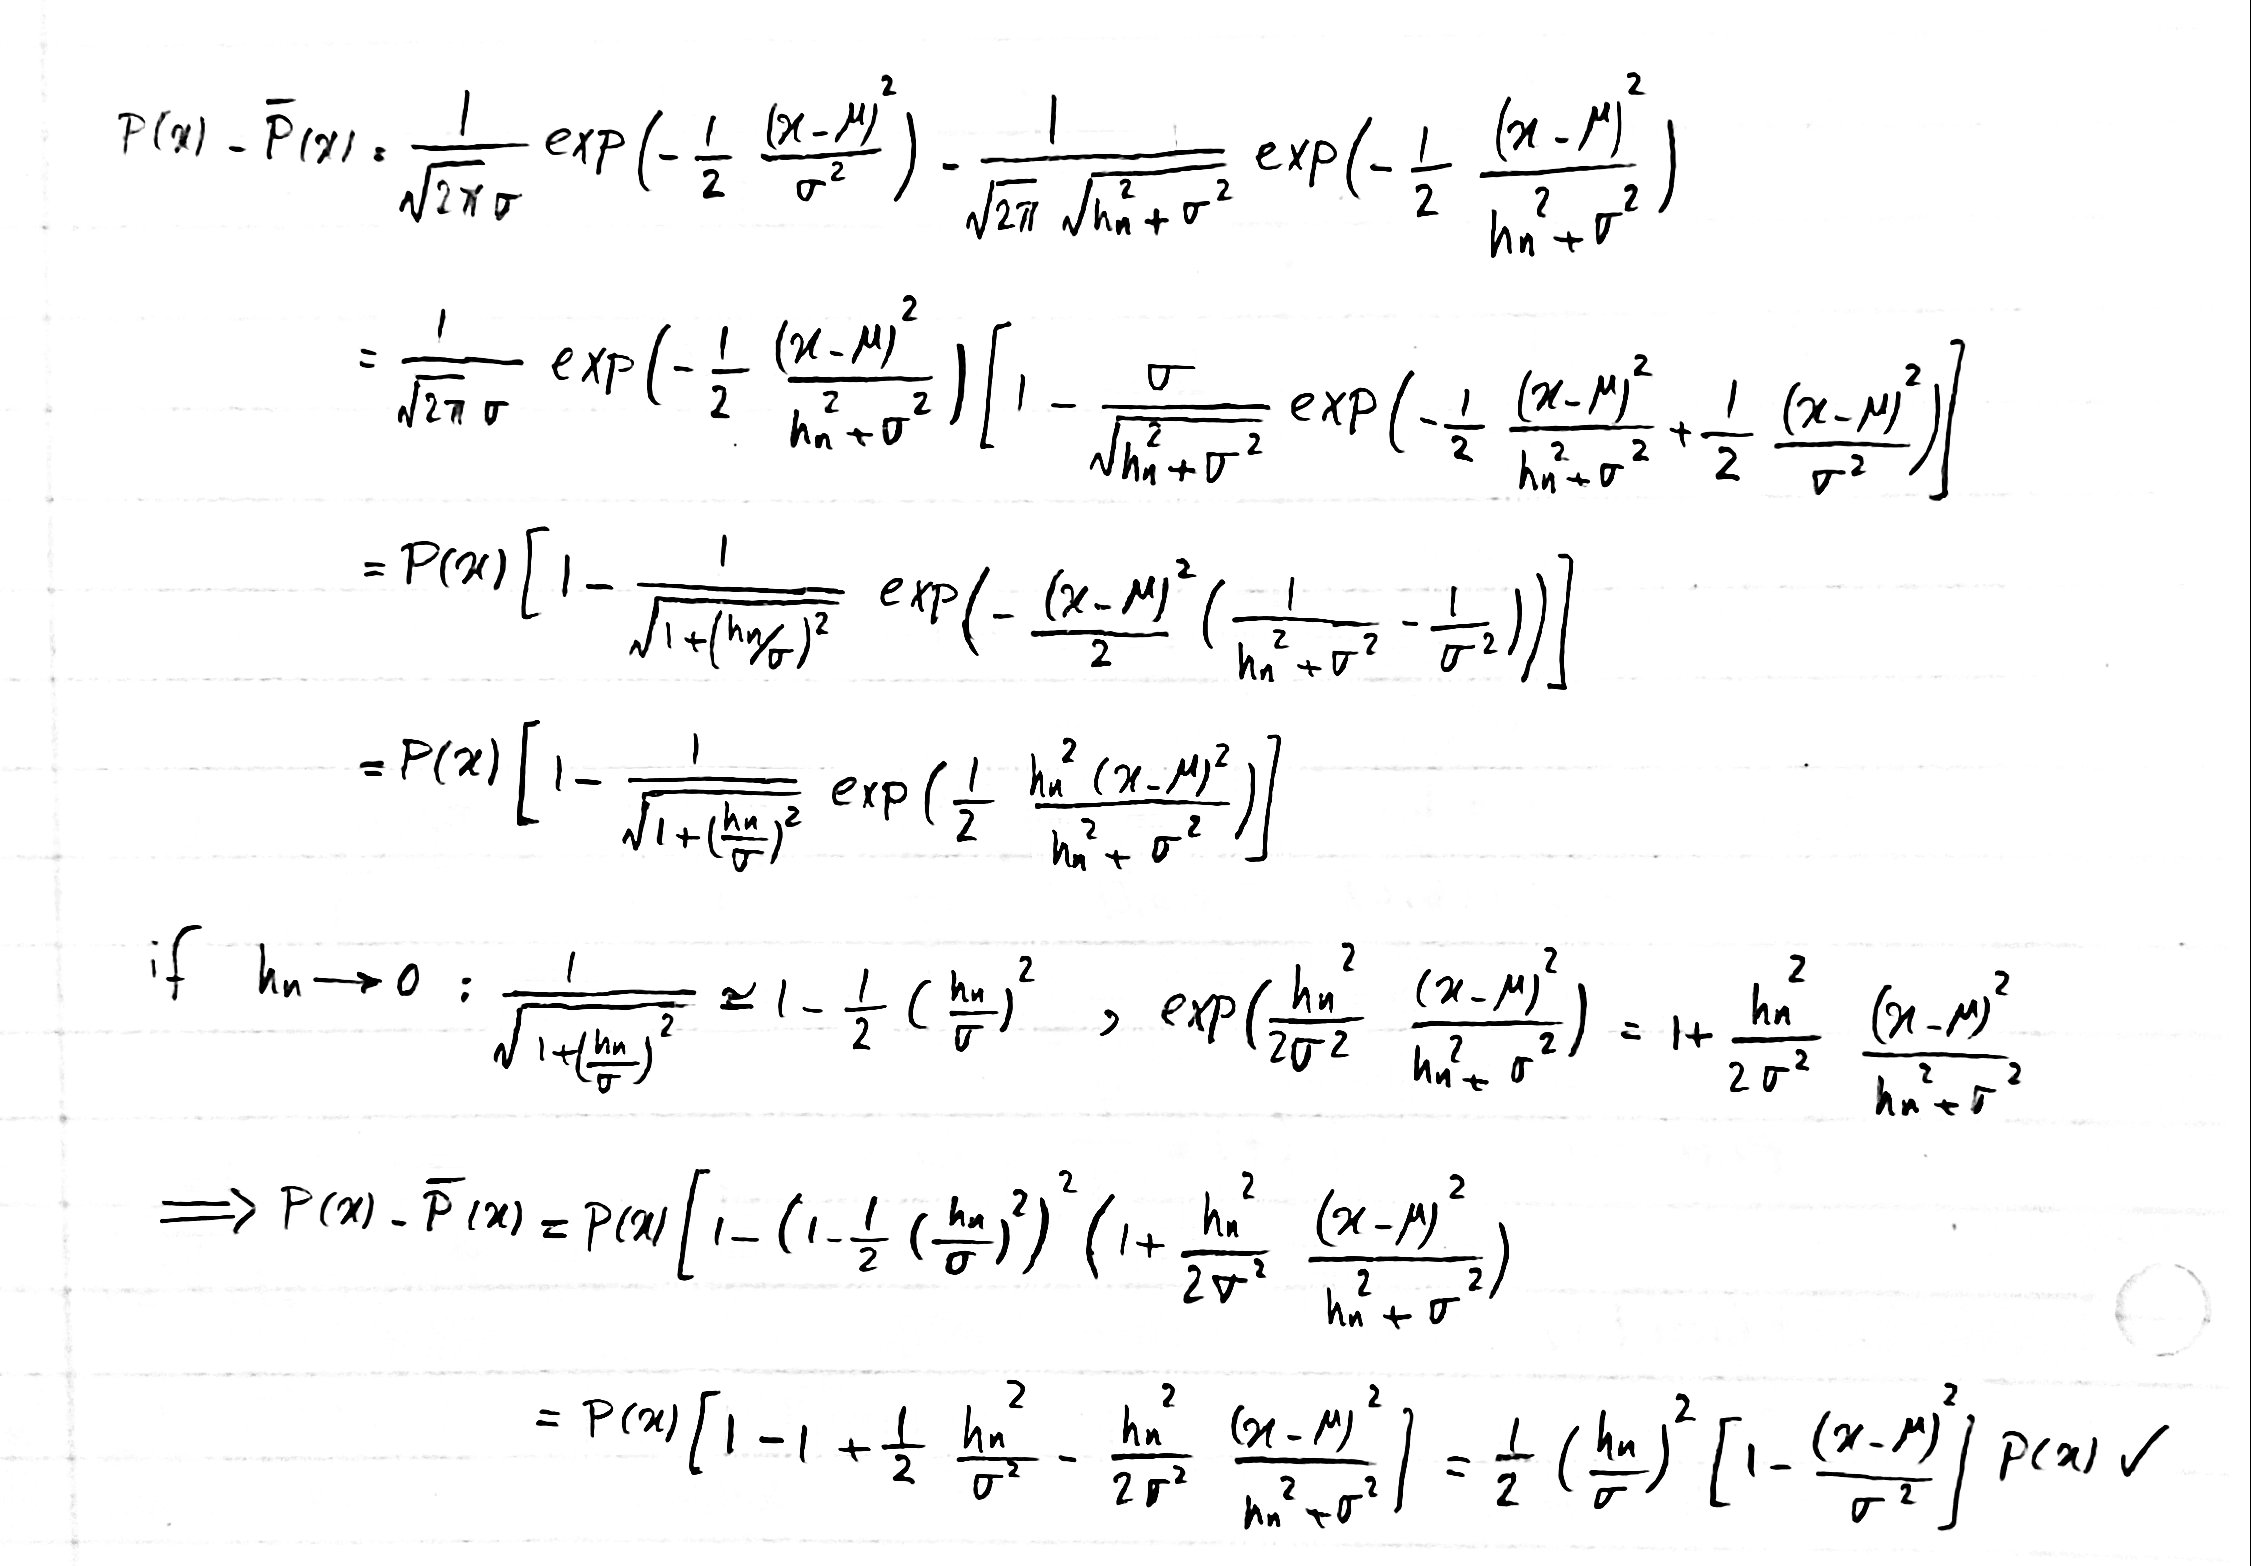
\includegraphics[width=\linewidth]{hand_written/32.jpg}
    \end{center}
\end{figure}
\newpage

\subsection*{ج}
\begin{figure}[h!]
    \begin{center}
    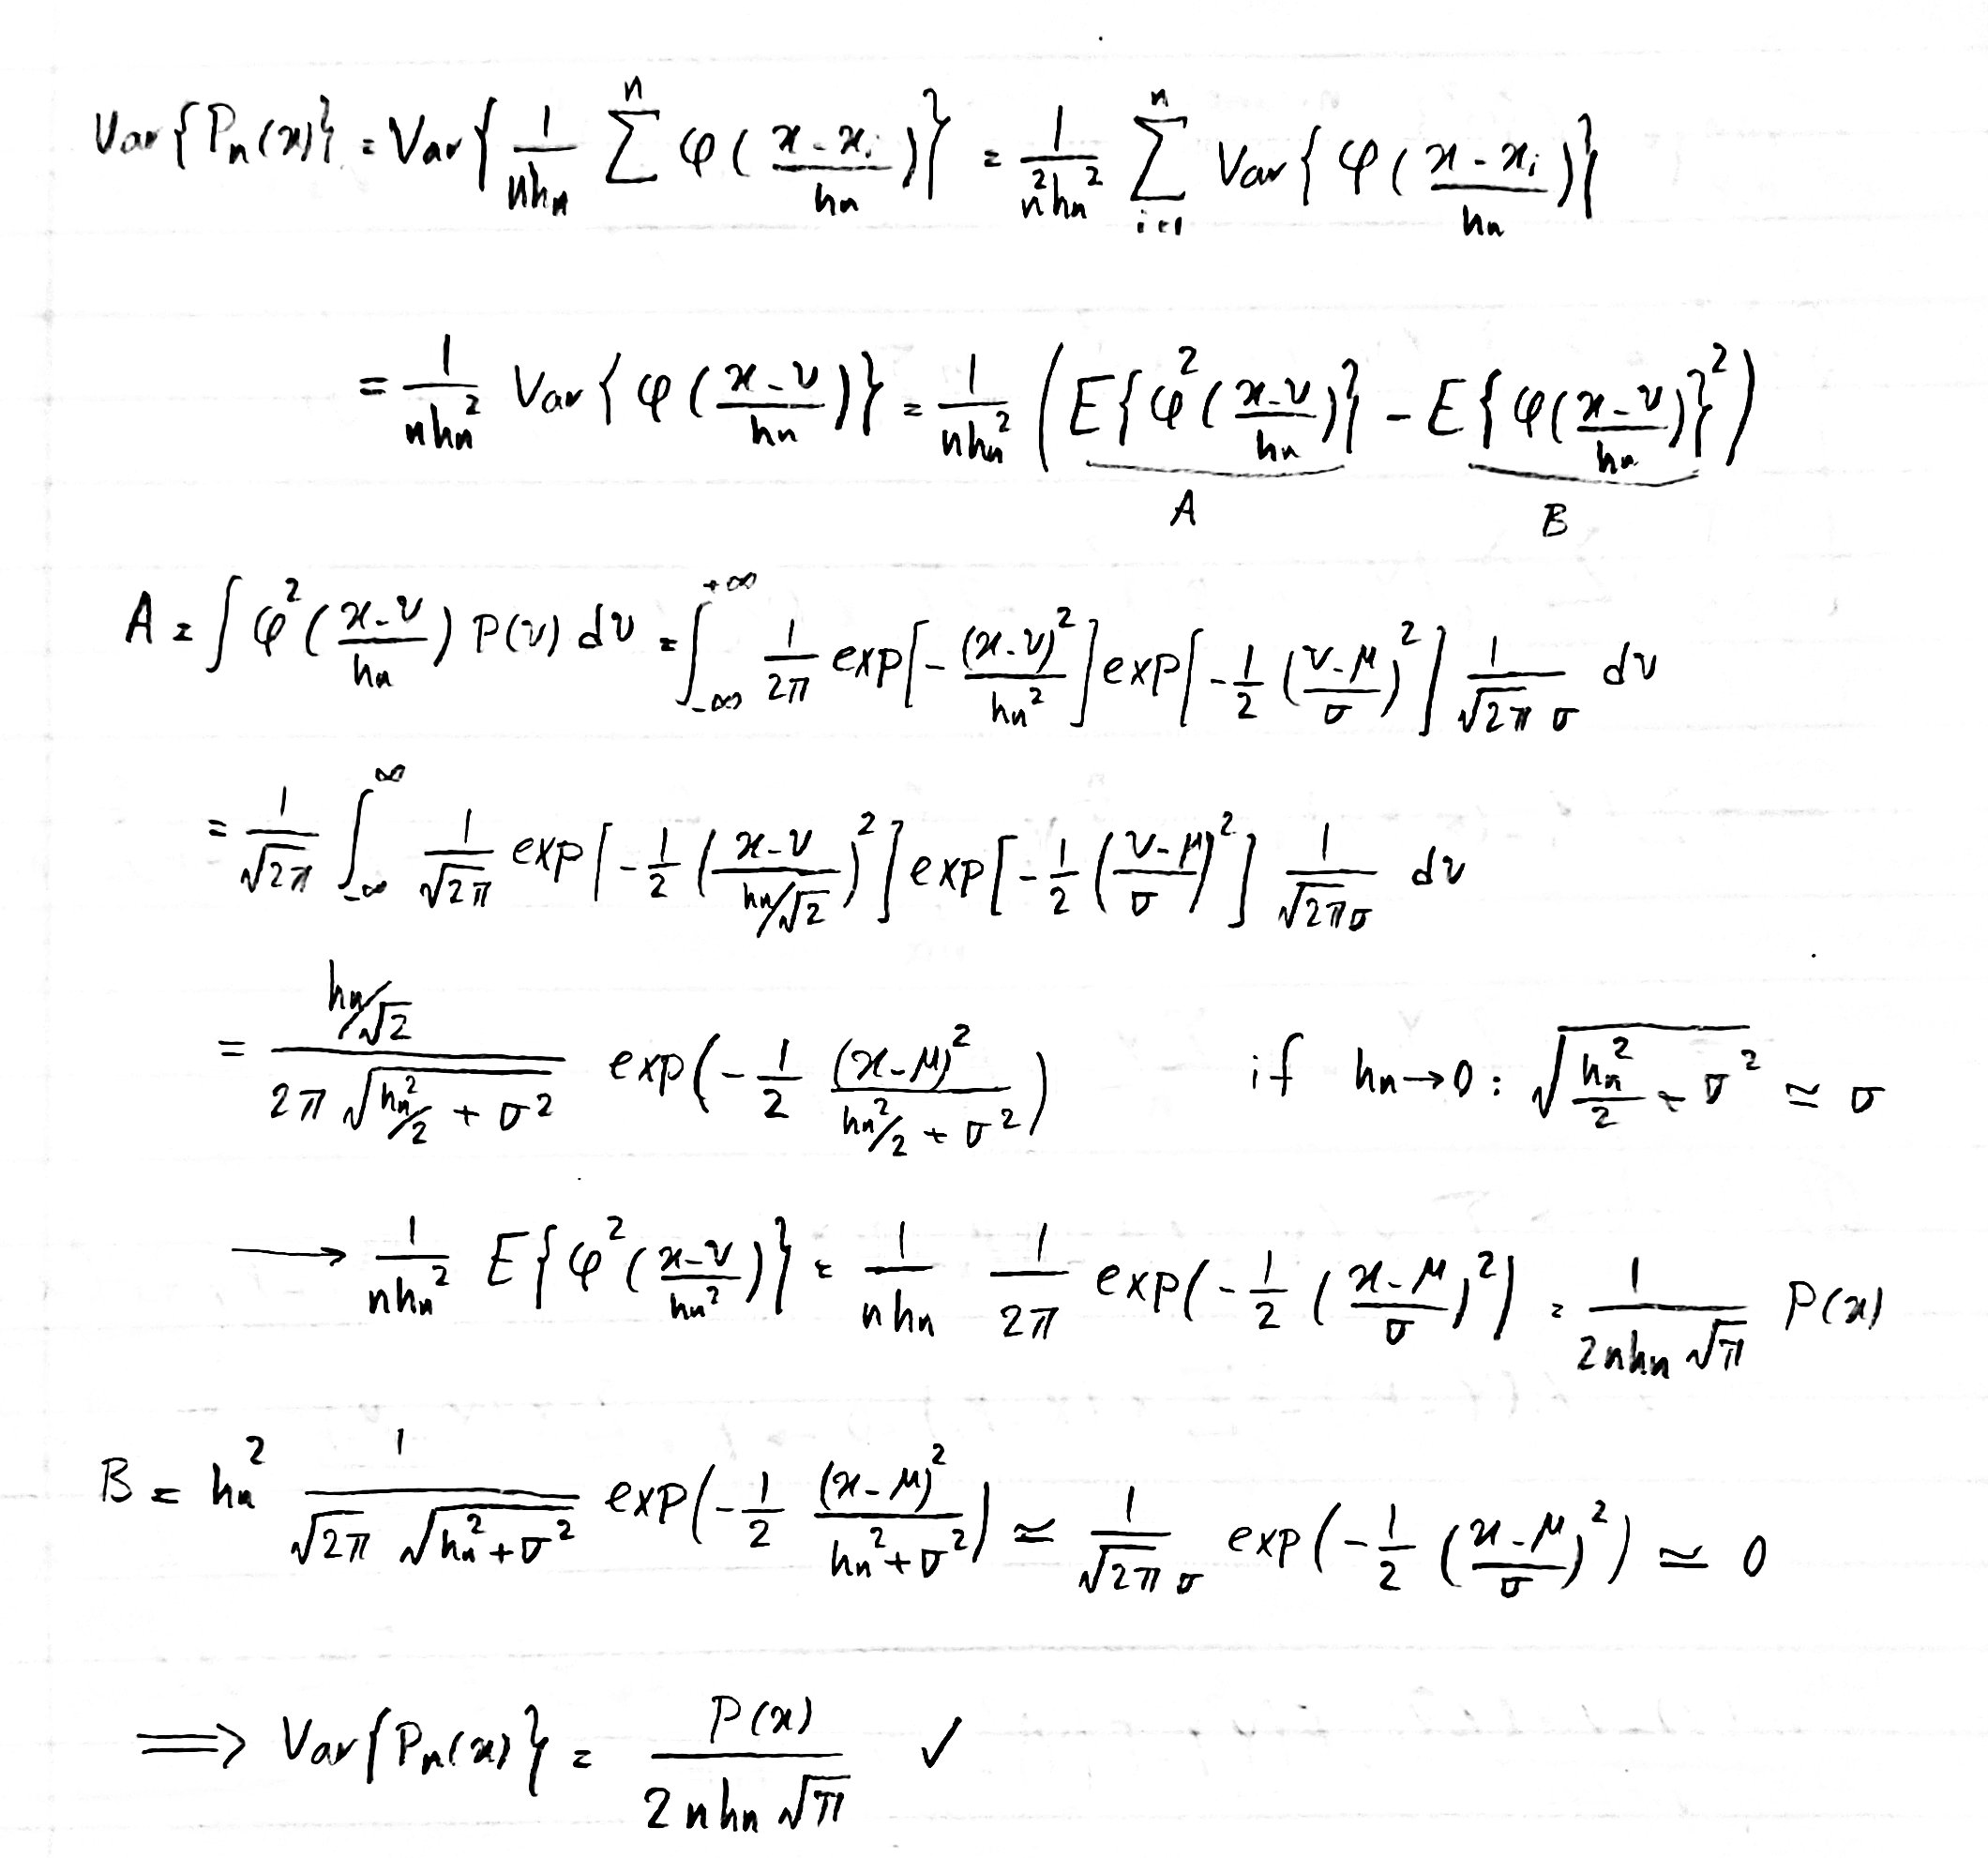
\includegraphics[width=\linewidth]{hand_written/33.jpg}
    \end{center}
\end{figure}
\newpage
\section{سوال چهار}
\begin{figure}[h!]
    \begin{center}
    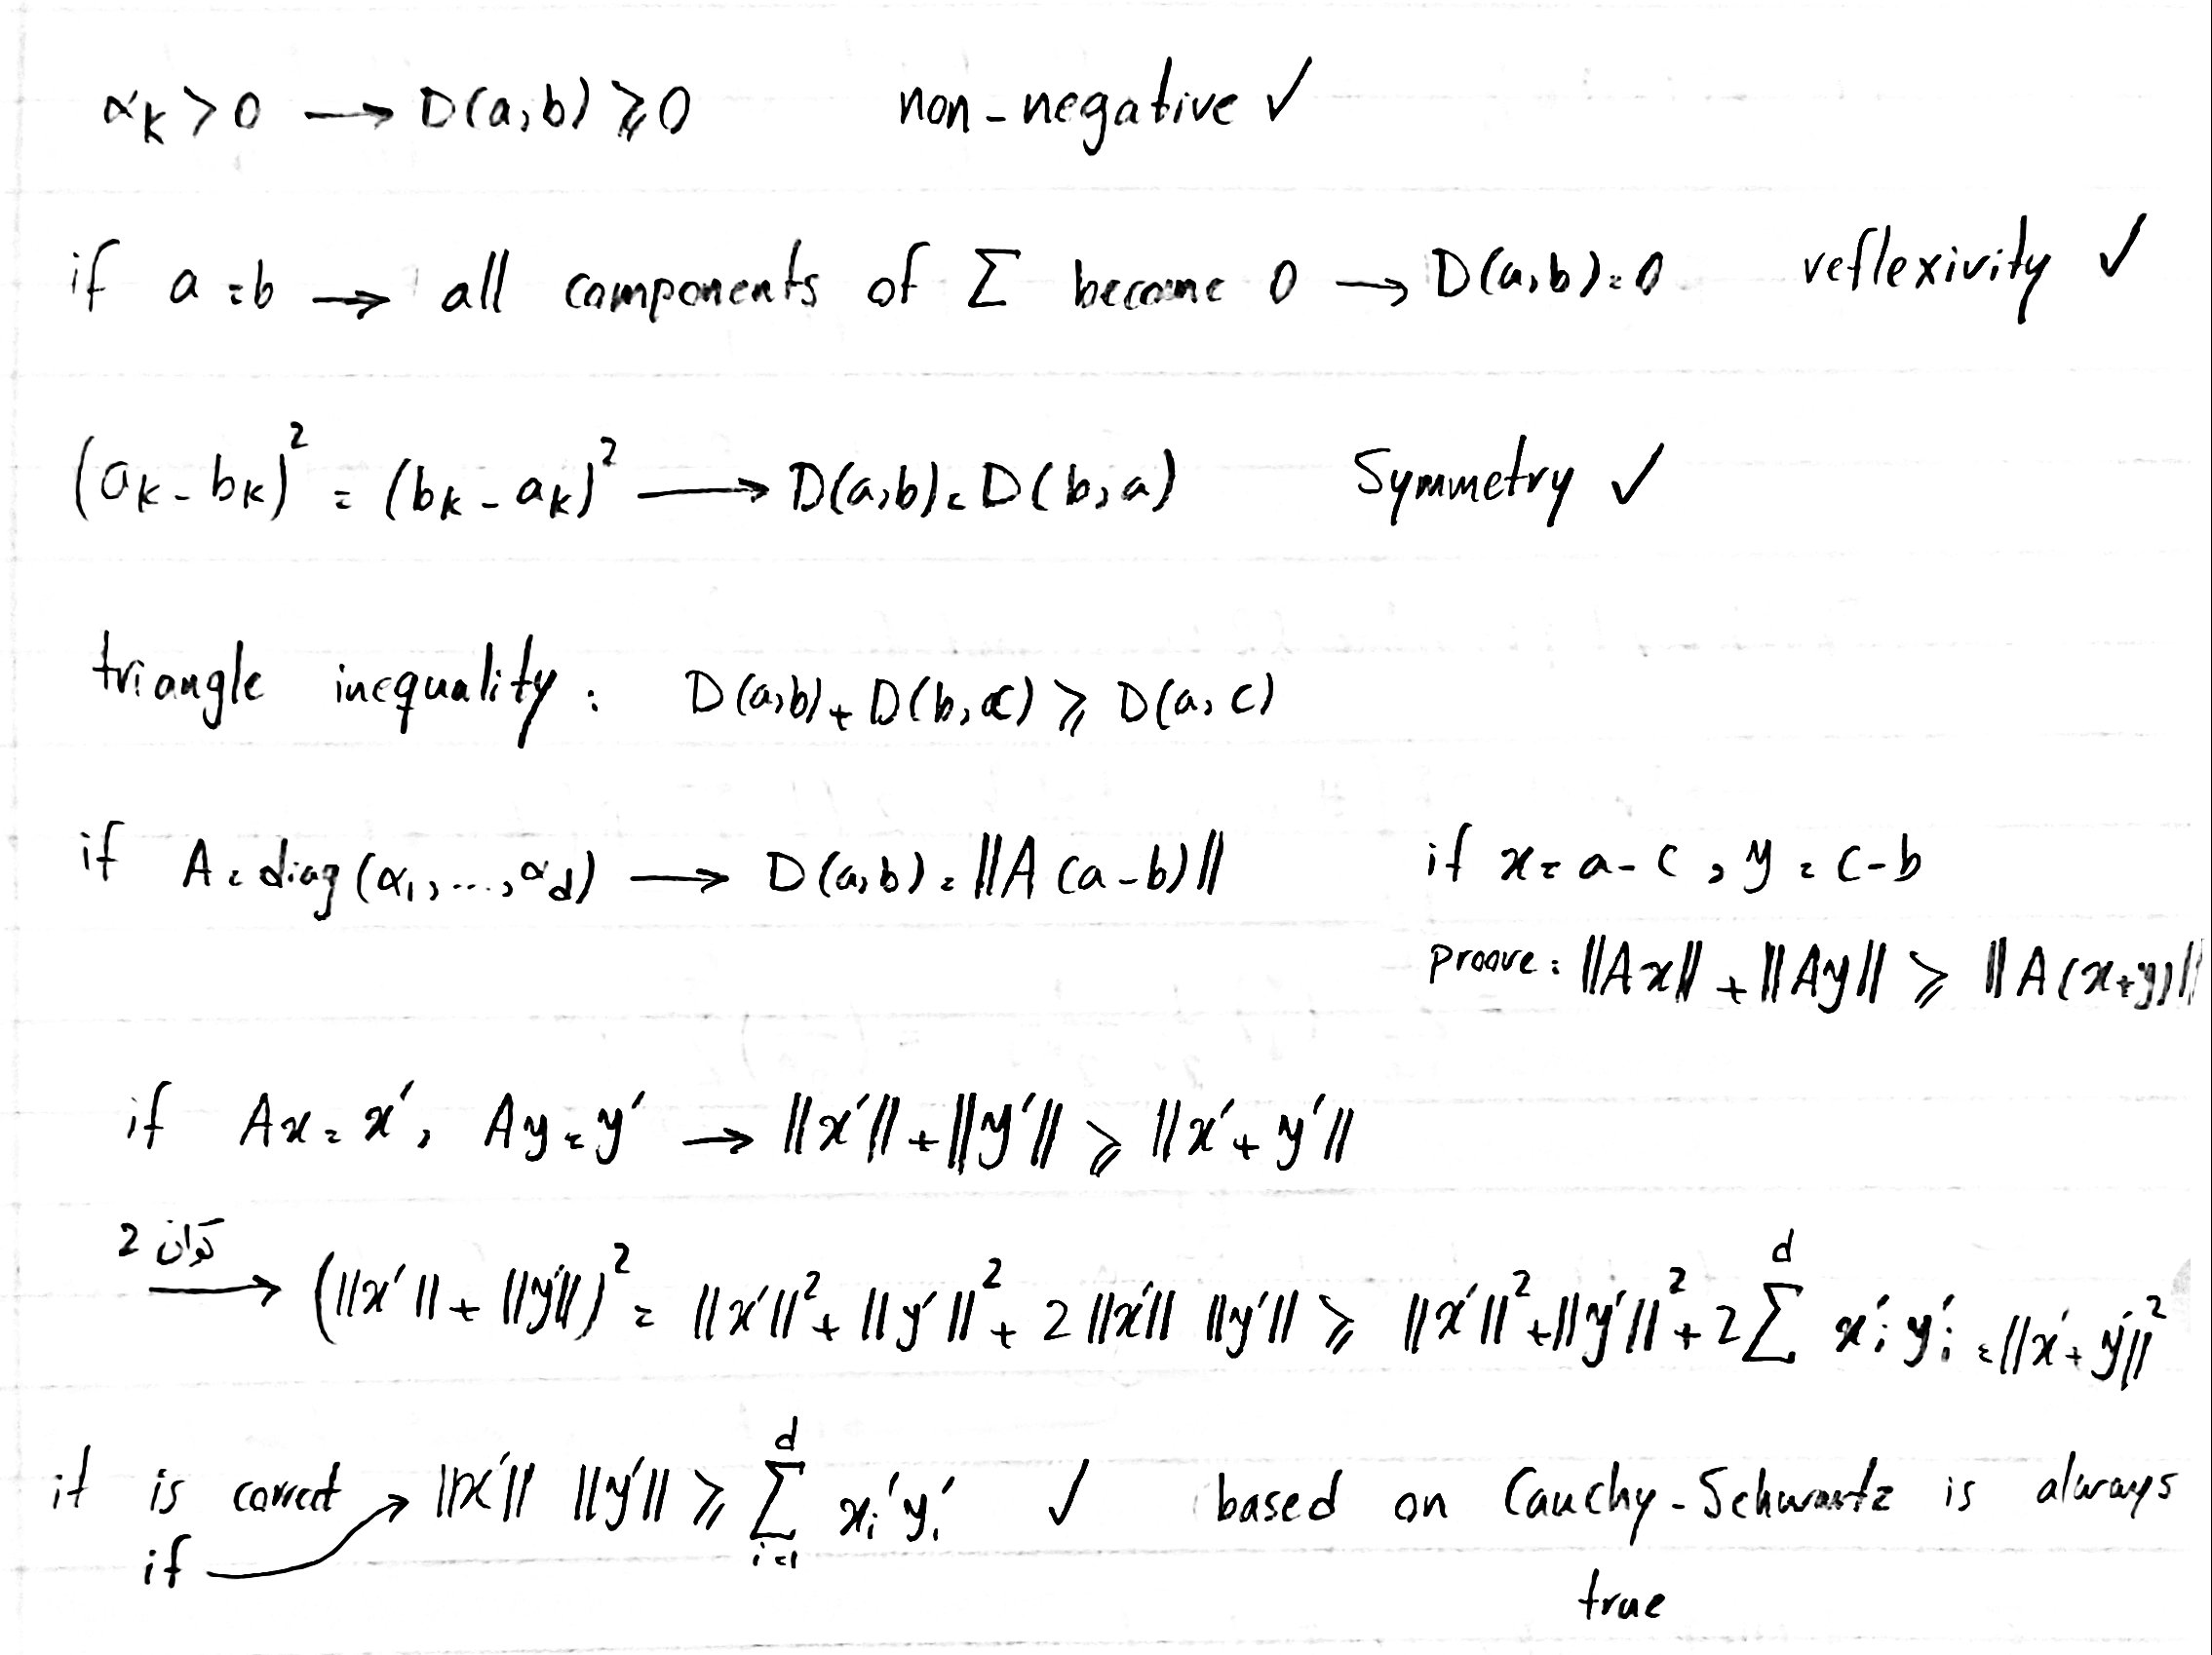
\includegraphics[width=\linewidth]{hand_written/4.jpg}
    \end{center}
\end{figure}

\newpage
\section{سوال پنج}
\begin{figure}[h!]
    \begin{center}
    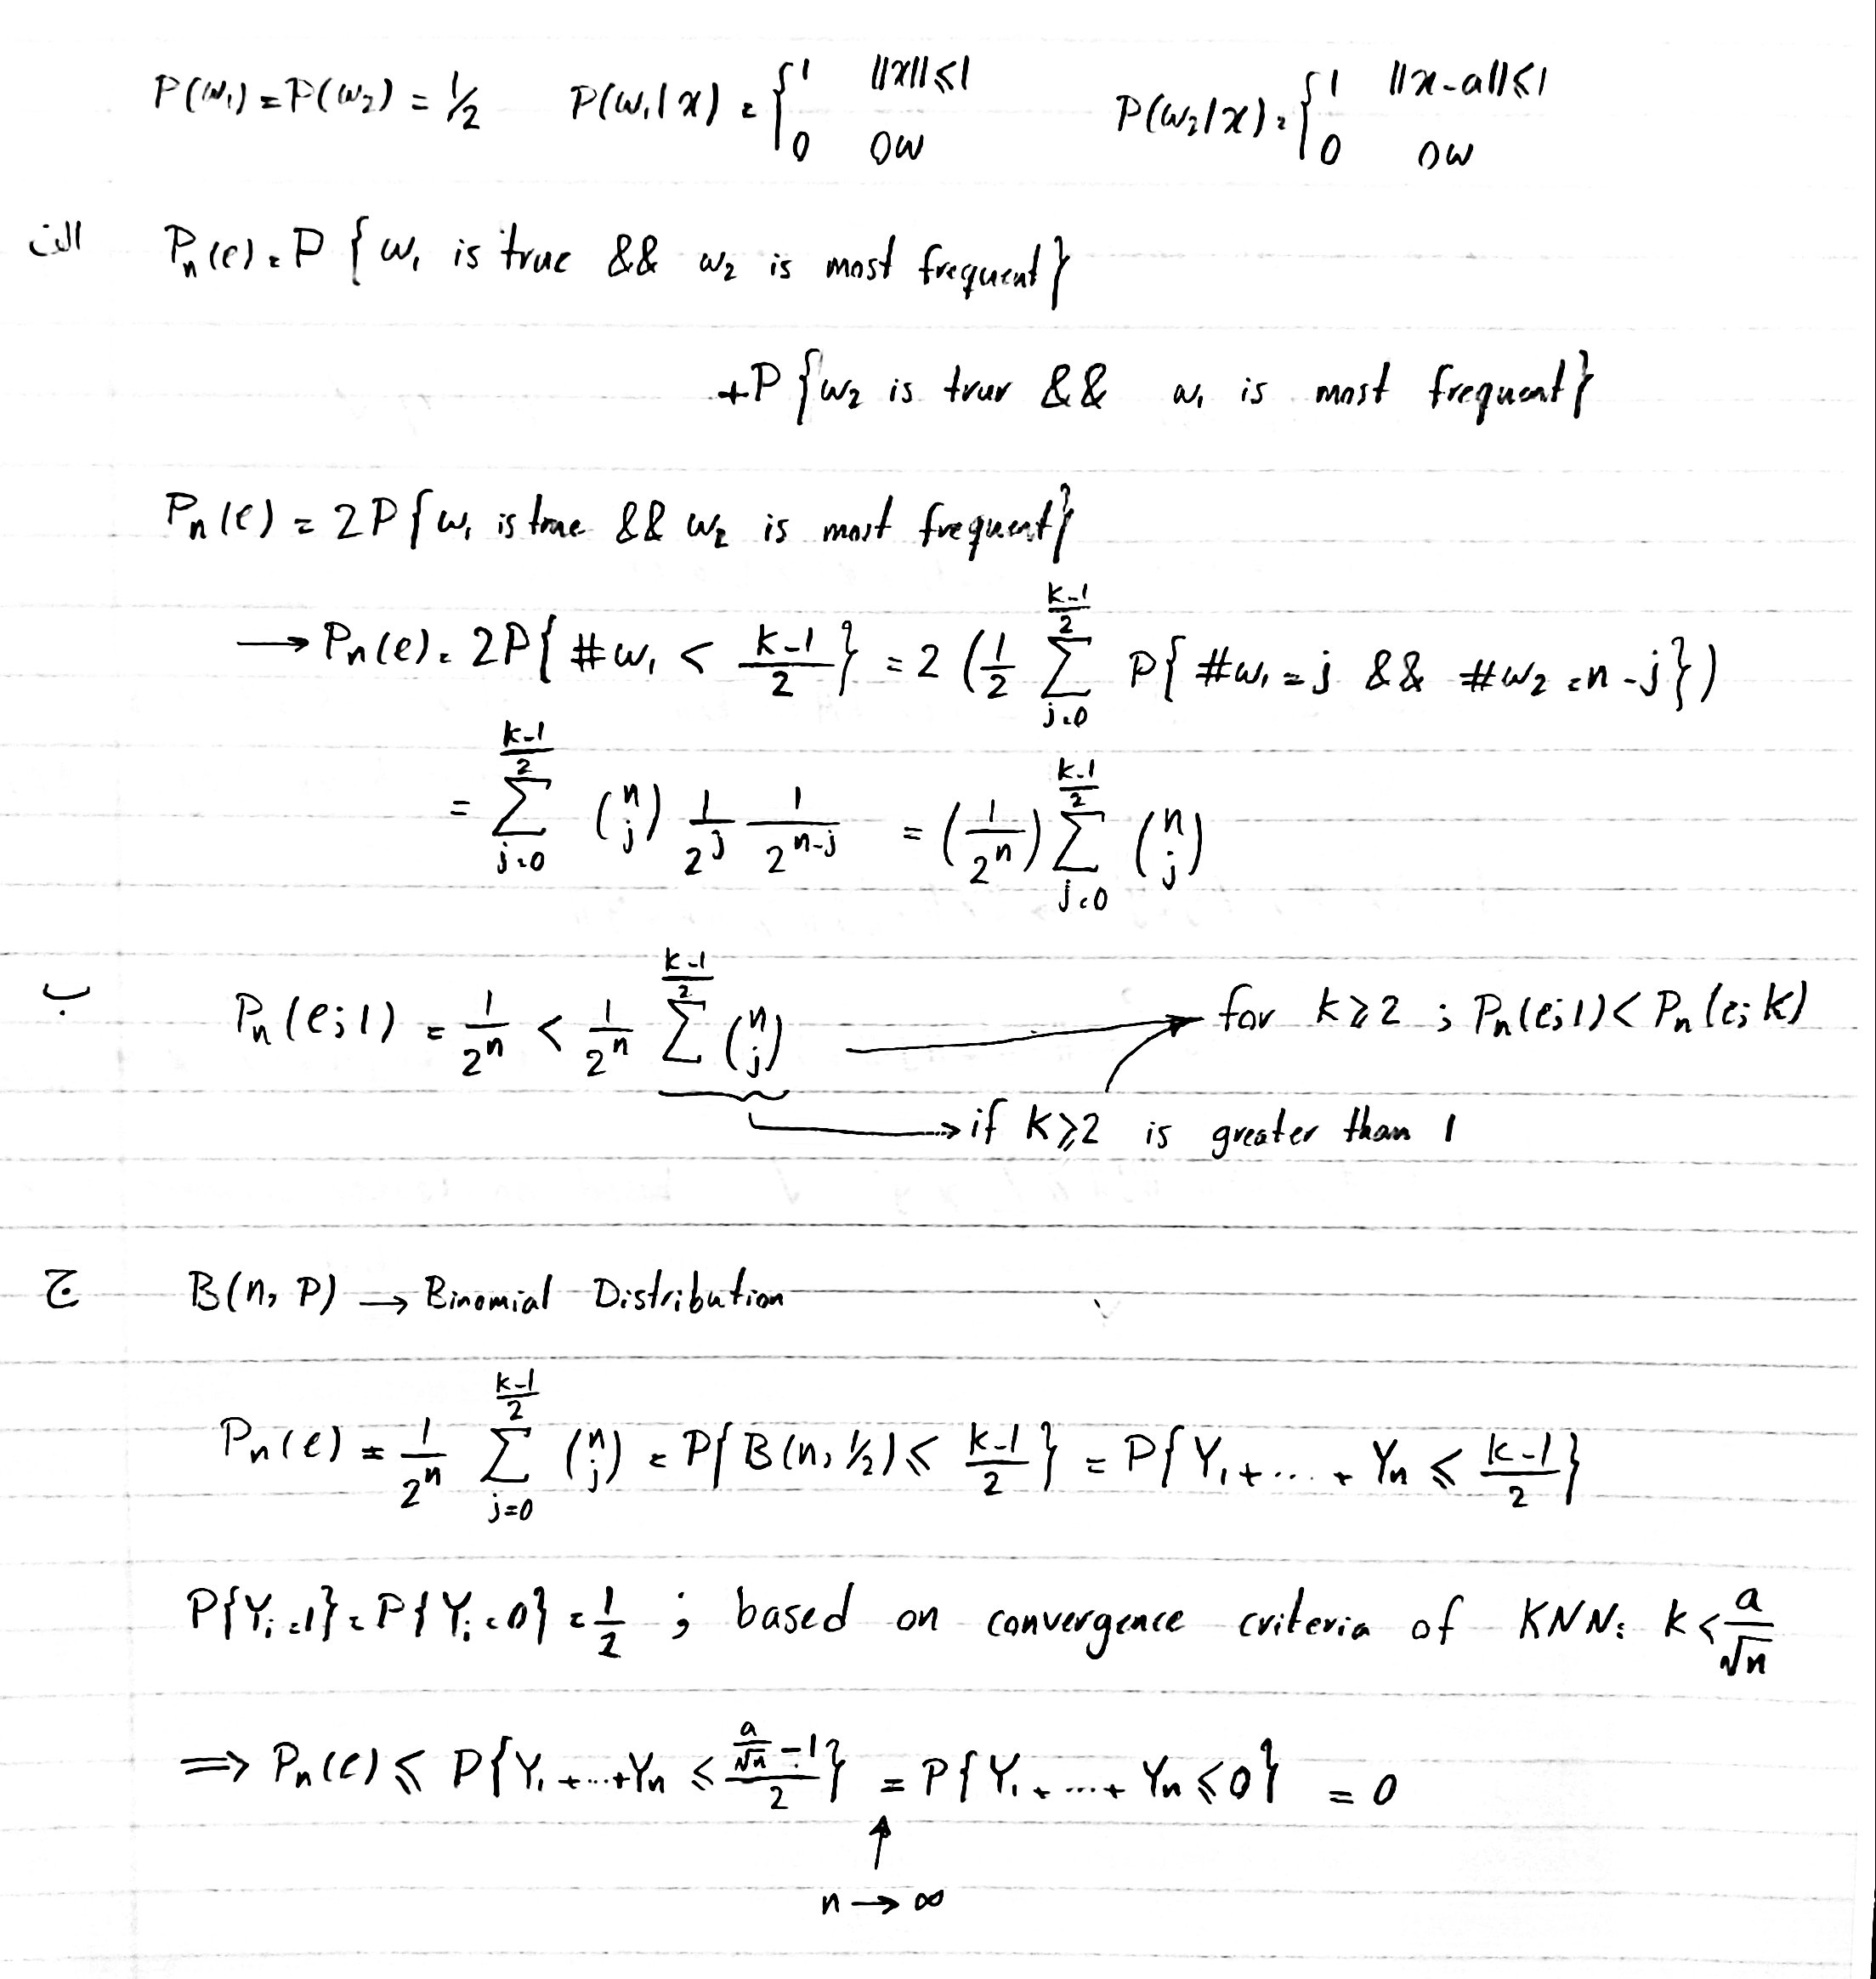
\includegraphics[width=\linewidth]{hand_written/5.jpg}
    \end{center}
\end{figure}

\newpage
\section{سوال شش (شبیه سازی)}
\subsection*{الف}

\begin{figure}[h!]
    \centering
    \subfigure[۵ بعدی]{
    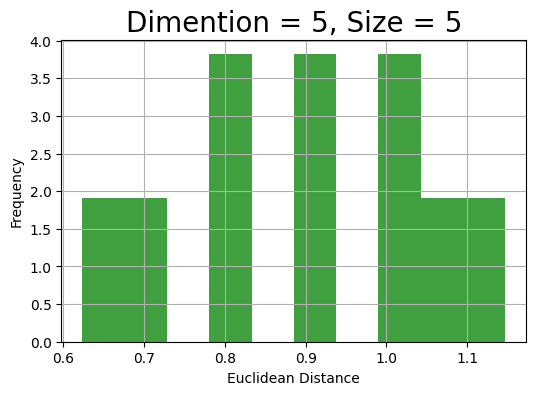
\includegraphics[width=.35\textwidth]{q6/a1.png}
    }
    \subfigure[۱۰ بعدی]{
    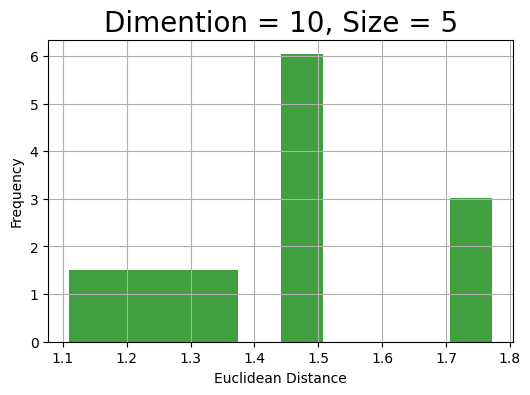
\includegraphics[width=.35\textwidth]{q6/a2.png}
    }
    \subfigure[۱۰۰ بعدی]{
    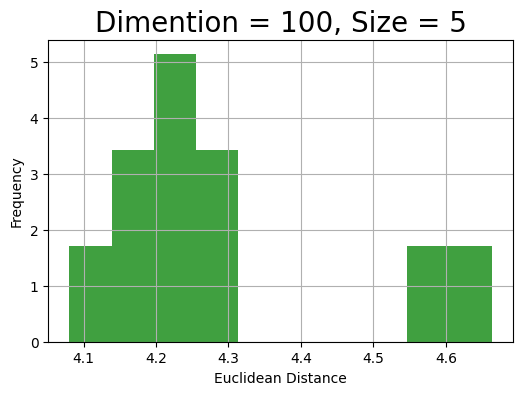
\includegraphics[width=.35\textwidth]{q6/a3.png}
    }
    \subfigure[۵۰۰ بعدی]{
    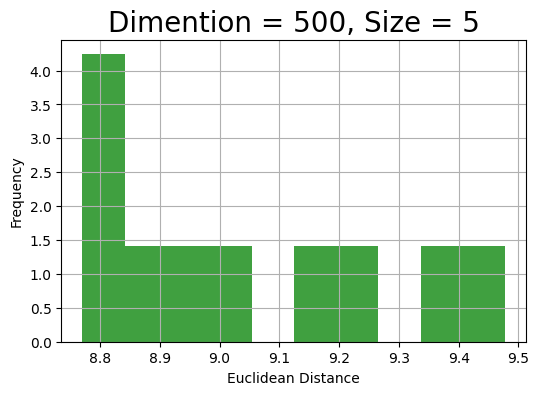
\includegraphics[width=.35\textwidth]{q6/a4.png}
    }
    \subfigure[۱۰۰۰ بعدی]{
    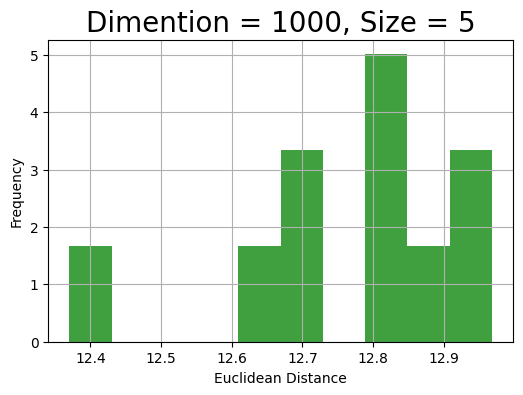
\includegraphics[width=.35\textwidth]{q6/a5.png}
    }
    \subfigure[۱۰۰۰۰ بعدی]{
    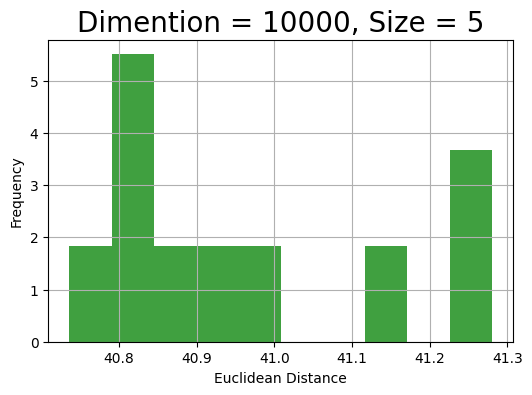
\includegraphics[width=.35\textwidth]{q6/a6.png}
    }
    \subfigure[۱۰۰۰۰۰ بعدی]{
    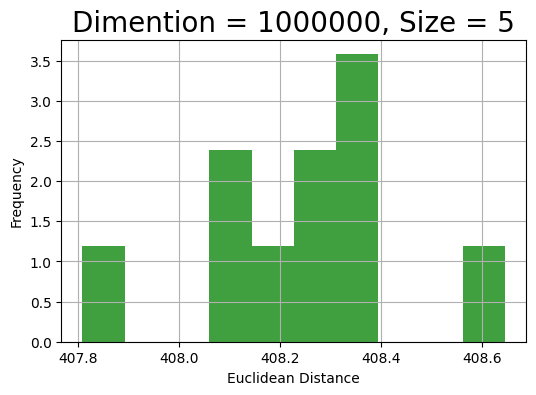
\includegraphics[width=.35\textwidth]{q6/a7.png}
    }
    \caption{خواسته‌های قسمت الف}
    \label{fig:9}
\end{figure}

در این سوال با استفاده از تابع رندوم کتابخانه \lr{numpy} و تابع \lr{hist} از کتابخانه \lr{matplotlib} هیستوگرام فاصله نقاط را به دست می‌آوریم. برا این کار تابع \lr{do task} پیاده سازی شده است که تعداد و بعد نقاط مورد نظر را در ورودی گرفته و نمودارها را رسم می‌کند.

\subsection*{ب}

\begin{figure}[h!]
    \centering
    \subfigure[5 نقطه]{
    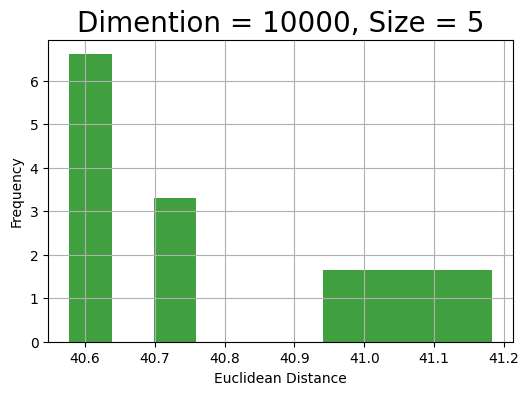
\includegraphics[width=.35\textwidth]{q6/b1.png}
    }
    \subfigure[۱۰ نقطه]{
    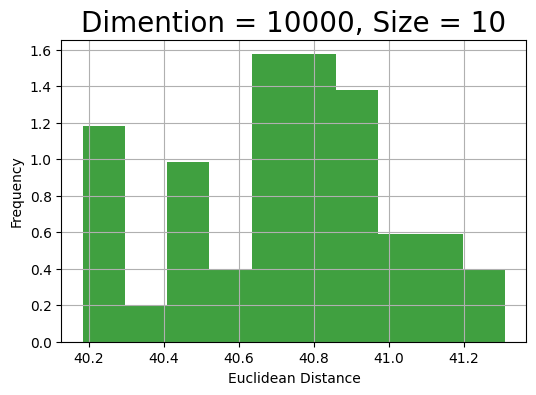
\includegraphics[width=.35\textwidth]{q6/b2.png}
    }
    \subfigure[۱۰۰ نقطه]{
    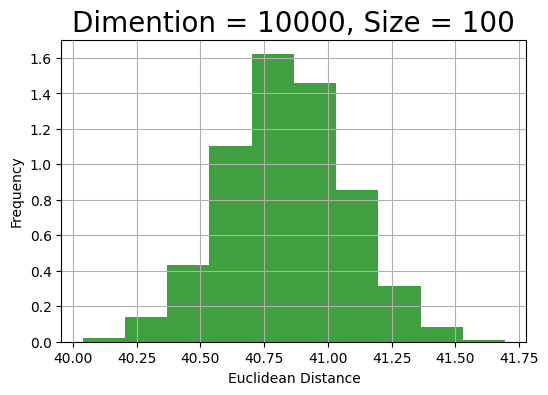
\includegraphics[width=.35\textwidth]{q6/b3.png}
    }
    \subfigure[۵۰۰۰ نقطه]{
    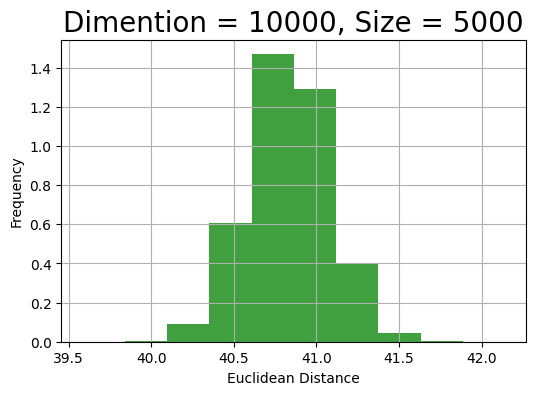
\includegraphics[width=.35\textwidth]{q6/b4.png}
    }
    \subfigure[۱۰۰۰۰ نقطه]{
    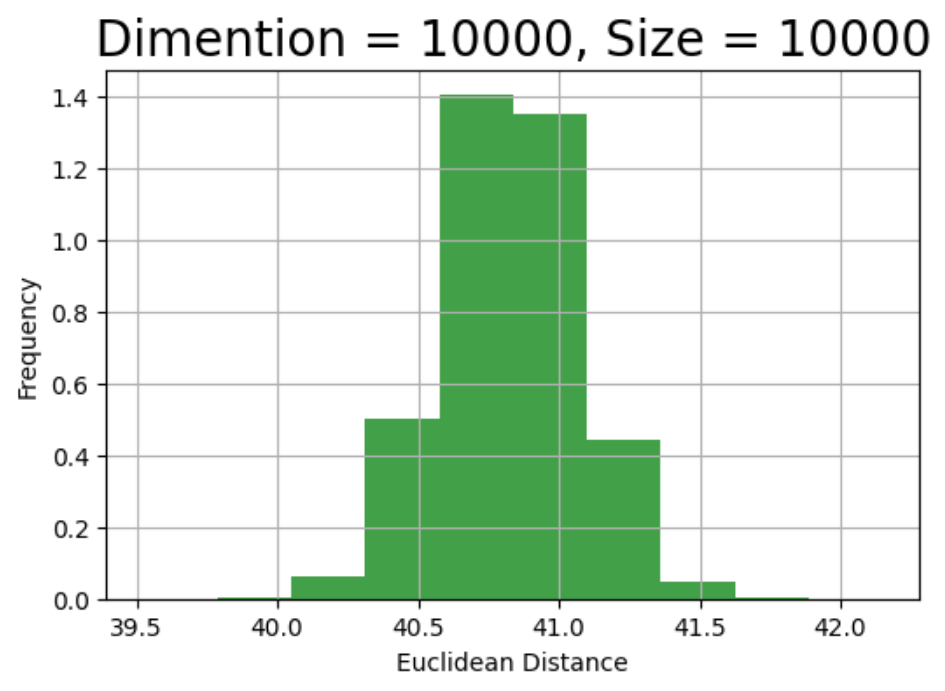
\includegraphics[width=.35\textwidth]{q6/b5.png}
    }
    \caption{خواسته‌های قسمت ب}
    \label{fig:10}
\end{figure}

\subsection*{ج}
اولین مسيله‌ای که به چشم می‌آید افزایش مدت زمان محاسبه فاصله نقاط از یکدیگر می‌باشد. همانطور که می‌دانیم پیچیدگی محاسباتی الگوریتم \lr{KNN} برابر با $O(mn)$ می‌باشد. (\lr{m} تعداد فیچر و \lr{n} تعداد داده‌های یادگیری می‌باشد.) یکی از مشکلات اساسی الگوریتم \lr{KNN} این است که در ابعاد بالا برای دقیق شدن تخمین باید تعداد داده‌ها را نیز افزایش دهیم که این موجب افزایش زمان طبقه بندی می‌شود. این مشکل همان نفرین ابعاد (\lr{curse of dimentionality}) است.


\newpage
\section{سوال هفت (شبیه سازی)}
در این سوال با استفاده از الگوریتم \lr{KNN} تصاویر اعداد دست نویس فارسی را طبقه بندی می‌کنیم.
\subsection*{الف}
برای لود کردن دیتا ست از روی فایل‌های \lr{cdb} از اسکریپت پایتون معرفی شده در لینک قرار داده شده در صورت سوال استفاده می‌کنیم. یکی از توابع موجود در این اسکریپت \lr{read hoda datset} می‌باشد. آرگومان‌های ورودی که آدرس فایل دیتاست و سایز تصاویر می‌باشد را مطابق توضیحات پیج گیت‌هاب به تابع می‌دهیم. آرگومان \lr{reshape} را نیز \lr{True} قرار می‌دهیم و آرگومان \lr{one hot} را \lr{False}، در این صورت فیچرها که پیکسل عکس‌های $32\times 32$ هستند فلت شده و لیبل‌ها نیز یک عدد بین ۰ و ۹ خواهند بود.\\
در شکل \ref{fig:1} سه نمونه از تصاویر متعلق به هر کلاس نمایش داده ‌شده‌اند. (رنگ‌ ها غیر واقی می‌باشند، تمام تصاویر یک کاناله و \lr{gray scale} هستند.)

\begin{figure}[h!]
    \begin{center}
    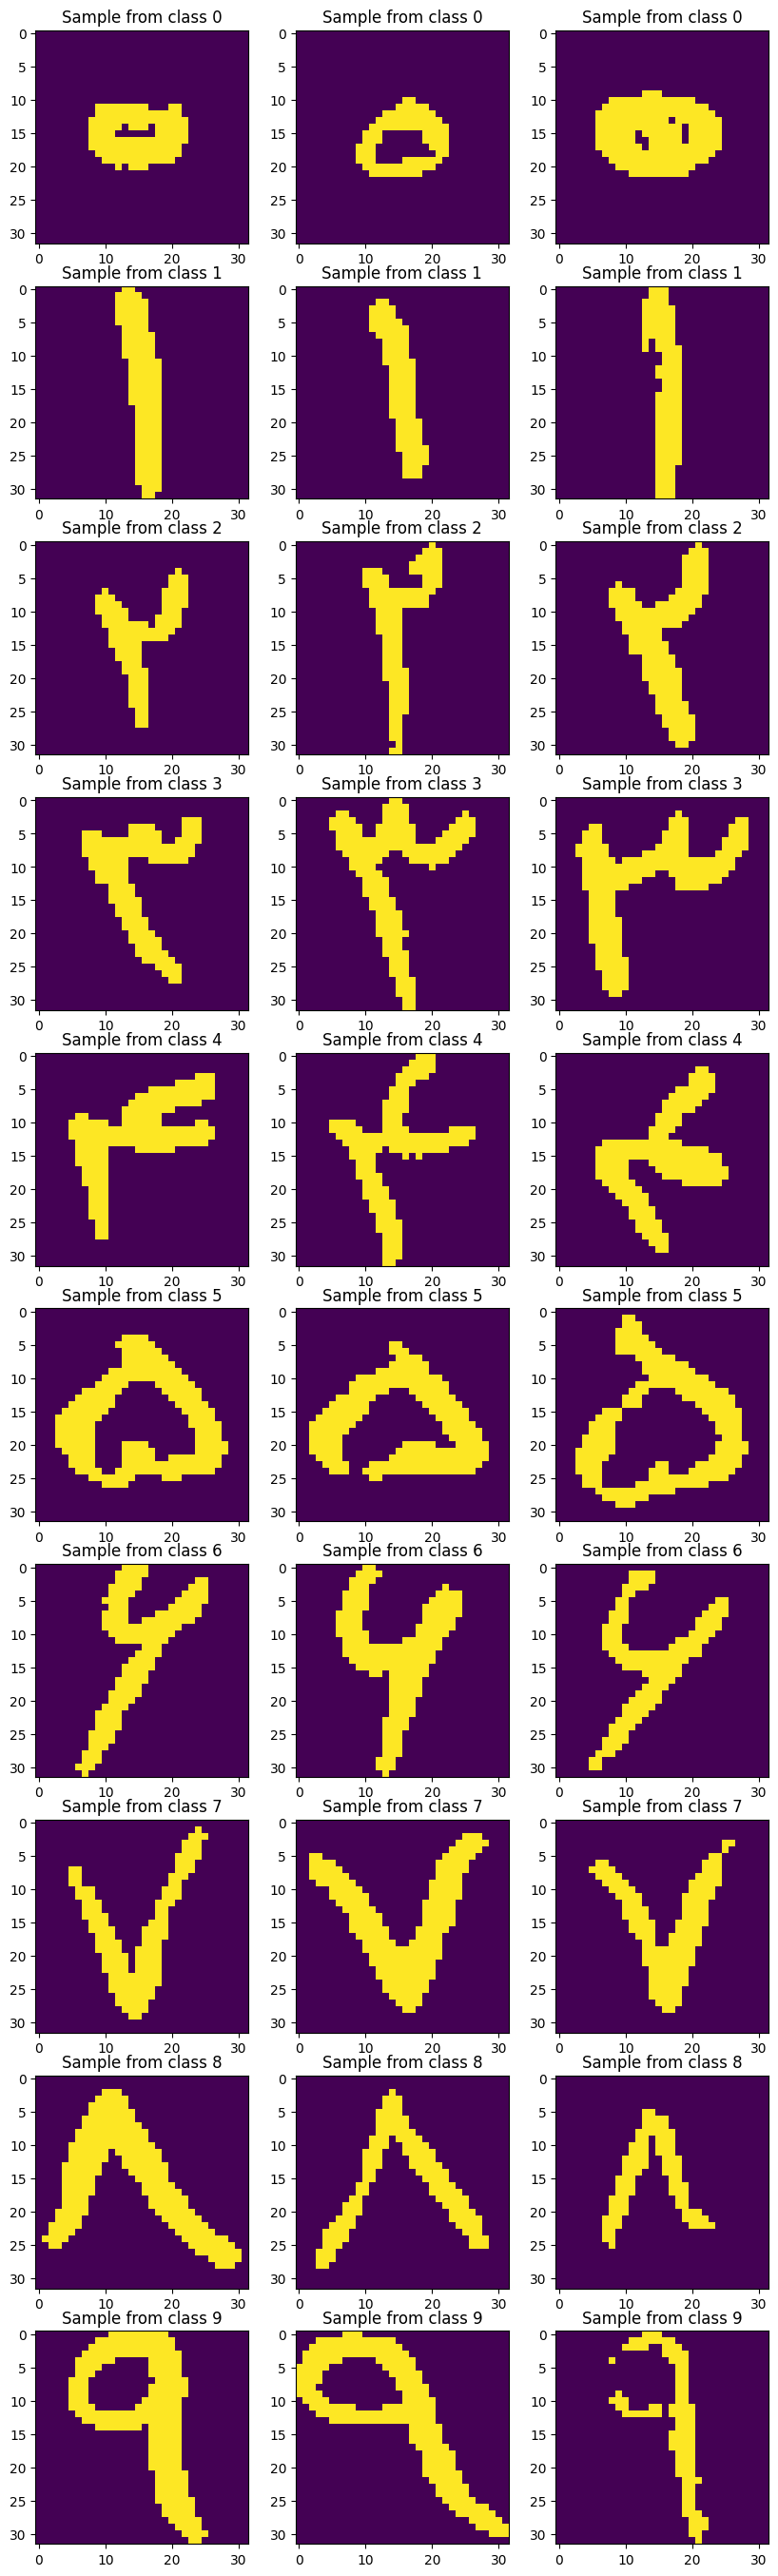
\includegraphics[scale=0.27]{q7/Q7_a.png}
    \caption{چند نمونه از تصاویر موجود در دیتاست}
    \label{fig:1}
    \end{center}
\end{figure}

\subsection*{ب}
در این قسمت الگوریتم \lr{KNN} را به صورت دستی پیاده سازی می‌کنیم. به این منظور یک کلاس به نام \lr{KNN} با سه متد زیر پیاده سازی شده‌است:
\begin{description}
    \item[$\bullet$] \lr{constructor}: این تابع تنها هایپر پارامتر مدل که همان \lr{k} یا تعداد همسایه‌ها می‌باشد را به همراه دیتاست و فیچرها می‌گیرد و در متغییرهای کلاس ذخیره می‌کند. تعداد سمپل‌ها و ابعاد فیچر نیز از دیگر متغییرهای این کلاس هستند که از روی ورودی‌های این تابع به دست می‌آیند. لازم به ذکر است که ورودی‌های مربوط به سمپل‌ها و لیبل‌ها باید آرایه \lr{numpy} باشند.
    \item[$\bullet$] \lr{dist}: این تابع بع صورت برداری فاصله اقلیدسی دو بردار که آرگومان‌ها ورودی آن هستند را حساب می‌کند.
    \item[$\bullet$] \lr{predict}: در این تابع برای هر سطر از متغییر ورودی (\lr{x}) تخمین نان‌پارامتریک مدل را به دست می‌آوریم. ابتدا با استفاده از متد \lr{dist} و تابع \lr{argsort} کتابخانه \lr{numpy} همسایه‌های نقاط را به دست می‌آوریم. در نهایت با استفاده از تابع \lr{unique} و \lr{argmax} پر تکرارترین لیبل در بین \lr{k}همسایه نزدیک نقطه مورد بررسی را به دست آورده و آن نقطه را در همان طبقه قرار می‌دهیم. 
\end{description}
سرعت محاسبه تابع \lr{predict} در مقایسه با توابع آماده کتابخانه \lr{scikit learn} به مقدار قابل توجهی کمتر است. لیبل کردن ۲۰۰۰۰ دیتا از مجموعه تست حدودا ۳۰ دقیقه زمان برد. نتایج طبقه بندی در جدول \ref{table:1} و شکل \ref{fig:2} آورده شده است.

\begin{table}[h!]
    \begin{tabular}{|c|c|c|c|c|c|c|c|c|c|c|}
    \hline
    $9$     & $8$     & $7$     & $6$     & $5$     & $4$     & $3$     & $2$     & $1$     & $0$     & \lr{label}    \\ \hline
    $96.30$ & $97.77$ & $98.69$ & $97.63$ & $97.10$ & $94.33$ & $89.28$ & $88.82$ & $94.37$ & $98.83$ & \lr{F1 Score} \\ \hline
    \end{tabular}
    \caption{نتایج طبقه بندی \lr{KNN} با داده‌های نرمالایز نشده}
    \label{table:1}
\end{table}

\begin{figure}[h!]
    \begin{center}
    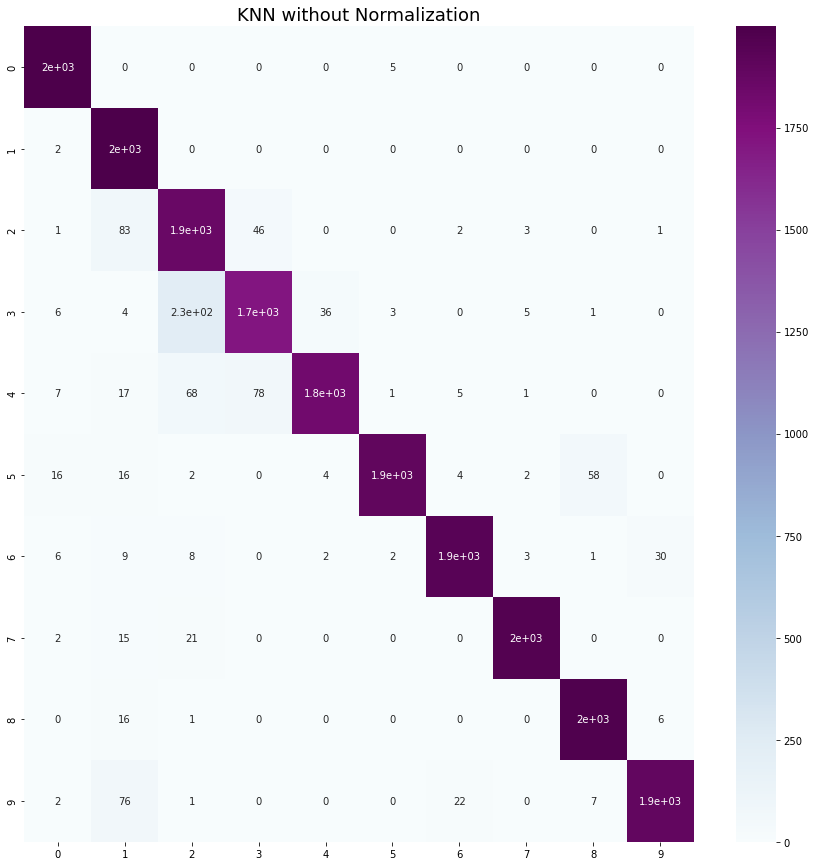
\includegraphics[scale=0.5]{q7/Q7_b1.png}
    \caption{\lr{Confusion Matrix} طبقه بند \lr{KNN} با داده‌های نرمالایز نشده}
    \label{fig:2}
    \end{center}
\end{figure}
همانطور که از ماتریس آشفتگی و \lr{f1 score} نیز مشخص است، دقت تمایز بین برخی کلاس‌ها پایین تر است. برای نمونه اعداد ۲ و ۳ فارسی شباهت زیادی به یک دیگر دارند و در مجموعه تست تعدادی از نمونه‌های این دو کلاس اشتباه طبقه بندی شده‌اند. کلاس ۹ و ۱ نیز تعداد اشتباه به نسبت بالایی دارند.

\subsection*{ج}
در این قسمت بردار فیچر را با استفاده از رابطه زیر نرمال می‌کنیم:
\begin{equation*}
    \mathbf{D} = \left\{\overrightarrow{x_{1}}, \overrightarrow{x_{2}}, \cdots , \overrightarrow{x_{n}}\right\} 
\end{equation*}
\begin{equation*}
    \overrightarrow{x_{i}} := \frac{\overrightarrow{x_{i}}}{\sum_{j = 1}^{d} x_{i}^{j} } 
\end{equation*}
با استفاده از رابطه فوق دو بردار \lr{X train} و \lr{X test} نرمال شده و در آزایه‌ی جدیدی ذخیره می‌کنیم و مجداداً عکس‌ها را طبقه‌بندی می‌کنیم. نتایج طبقه بندی با داده‌های نرمال شده بر روی مجموعه تست در شکل \ref{fig:3} نشان داده شده است.
\begin{figure}[h!]
    \begin{center}
    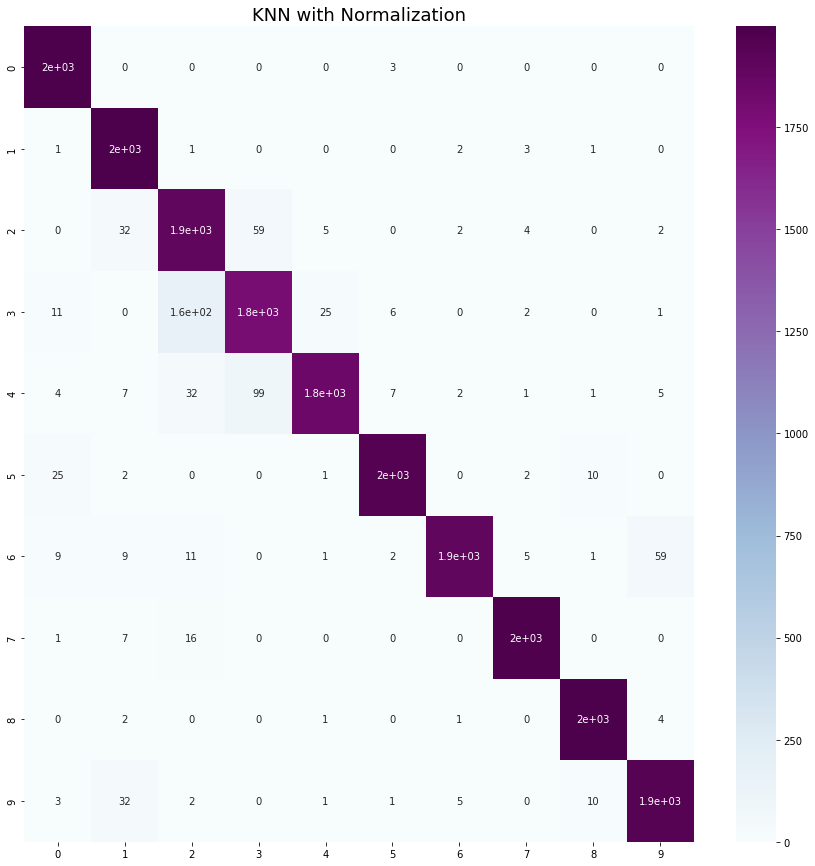
\includegraphics[scale=0.5]{q7/Q7_b2.png}
    \caption{\lr{Confusion Matrix} طبقه بند \lr{KNN} با داده‌های نرمالایز شده}
    \label{fig:3}
    \end{center}
\end{figure}

از ماتریس آشفتگی و جدول \ref{table:2} می‌توان نتیه گرفت که در مقایسه با نتایج قسمت قبل بهبود اندکی در عملکرد طبقه بند به چشم می‌خورد. 
\\
در تمامی قسمت‌های این تمرین از تعداد همسایه $K = 5$ در طبقه بند استفاده شده است.
\begin{table}[h!]
    \begin{tabular}{|c|c|c|c|c|c|c|c|c|c|c|}
    \hline
    $9$     & $8$     & $7$     & $6$     & $5$     & $4$     & $3$     & $2$     & $1$     & $0$     & \lr{label}    \\ \hline    
    $96.30$ & $97.77$ & $98.69$ & $97.63$ & $97.10$ & $94.33$ & $89.28$ & $88.82$ & $94.37$ & $98.83$ & \lr{F1 Score (Raw)}        \\ \hline
    $96.88$ & $99.22$ & $98.97$ & $97.21$ & $98.51$ & $95.04$ & $90.67$ & $91.97$ & $97.57$ & $98.59$ & \lr{F1 Score (Normal)} \\ \hline
    \end{tabular}
    \caption{مقایسه عملکرد طبقه‌بند \lr{KNN} با داده‌های پردازش نشده و داده‌های نرمال شده}
    \label{table:2}
\end{table}
\subsection*{د}
در این قسمت با استفاده از کلاس آماده \lr{KNeighborsClassifier} از کتابخانه \lr{Scikit Learn} طبقه بندی را برای داده‌های پردازش نشده و پردازش شده انجام می‌دهیم.
 عملکر طبقه بند با متریک \lr{F1 Score} و همچنین ماتریس‌های آشفتگی در شکل \ref{fig:4} و جدول \ref{table:3} نشان داده‌شده‌اند.
 \\برای ساخته نمونه از این کلاس تنها کافی است مقدار \lr{n neighbours} را در کانستراکتور تنظیم کنیم و سپس با استفاده از تابع \lr{fit} داده‌های یادگیری و لیبل آن‌ها را به آبجکت تشکیل شده بدهیم. در نهایت با استفاده از دستور \lr{predict} داده‌های تست را طبقه بندی کنیم.
 
\begin{figure}[h]
    \centering
    \subfigure[فیچرهای خام]{
    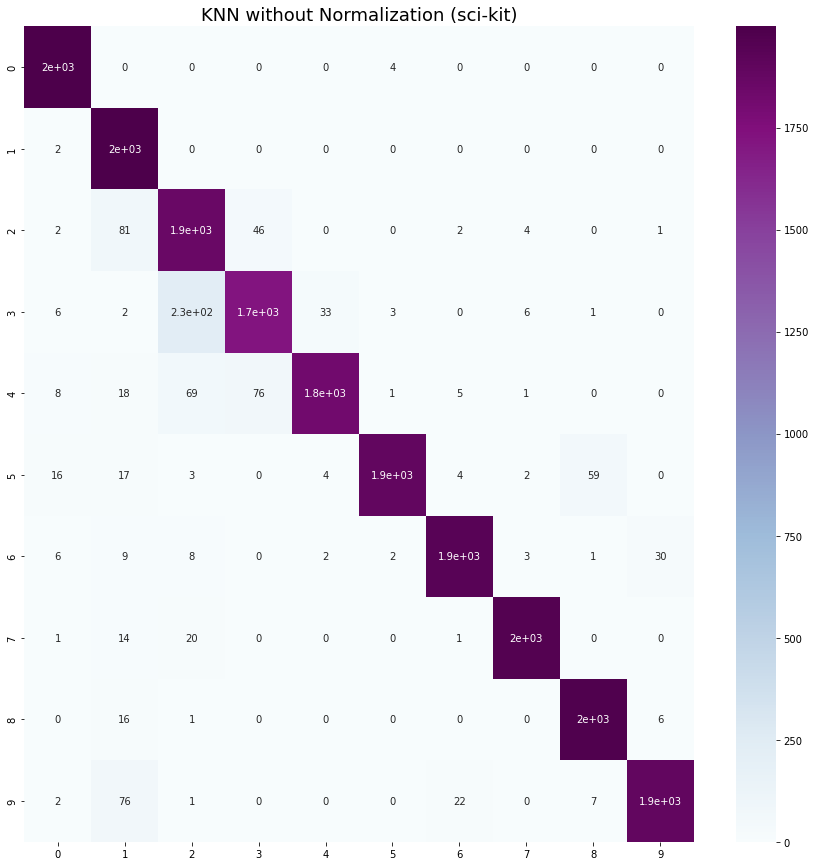
\includegraphics[width=.4\textwidth]{q7/Q7_d1.png}
    }
    \subfigure[فیچرهای نرمال شده]{
    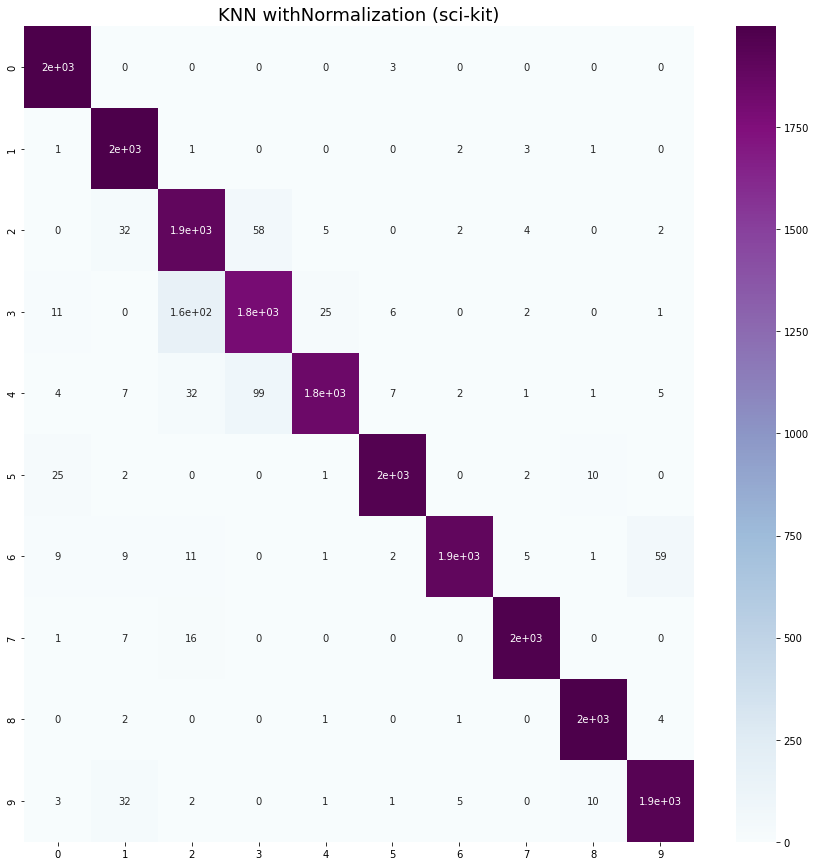
\includegraphics[width=.4\textwidth]{q7/Q7_d2.png}
    }
    \caption{طبقه بندی با کلاس کتابخانه \lr{scikit learn}}
    \label{fig:4}
\end{figure}

\begin{table}[h!]
    \begin{tabular}{|c|c|c|c|c|c|c|c|c|c|c|}
    \hline
    $9$     & $8$     & $7$     & $6$     & $5$     & $4$     & $3$     & $2$     & $1$     & $0$     & \lr{label}    \\ \hline
    $96.30$ & $97.75$ & $98.69$ & $97.60$ & $97.05$ & $94.37$ & $89.50$ & $88.84$ & $94.44$ & $98.83$ & \lr{F1 Score (Raw)} \\ \hline
    $96.88$ & $99.22$ & $98.97$ & $97.21$ & $98.51$ & $95.04$ & $90.70$ & $91.99$ & $97.57$ & $98.59$ & \lr{F1 Score (Normal)} \\ \hline
    \end{tabular}
    \caption{نتایج طبق بندی با استفاده از کتابخانه \lr{scikit learn}}
    \label{table:3}
\end{table}

\newpage
\section{سوال هشت (شبیه سازی)}
در این تمرین به پیاده سازی روش نان‌پارامتری پنجره پارزن می‌پردازیم. داده‌های موجود در فایل اکسل را با دستورات کتابخانه \lr{pandas} باز کرده و ستون \lr{duration} را در یک آرایه \lr{numpy} ذخیره می‌کنیم.
\\
برای پیاده سازی طبقه بند یک کلاس به نام \lr{parzen} پیاده سازی شده است. این کلاس چهار متد برای اجرای الگوریتم طبقه بندی و پیش بینی احتمال نقاط جدید دارد.

\begin{description}
    \item[$\bullet$] \lr{constructor}: برای ایجاد یک نمونه از این کلاس لازم است داده‌های یادگیری، نوع کرنل و اندازه پنجره برای فذاخوانی این تابع ارسال کرد. تعداد داده‌های یادگیری باید حتماً آرایه \lr{numpy} باشند.
    \item[$\bullet$] \lr{gaussian kernel}: این تابع با استفاده از رابطه $ \phi(\boldsymbol{x}) = \frac{1}{(\sqrt{2 \pi})^{d} h_{n}^{d}} \exp \left[-\frac{1}{2}\left(\frac{\boldsymbol{x}-\boldsymbol{x}_{i}}{h_{n}}\right)^{2}\right]$ کرنل گوسی را برای بردار ورودی حساب می‌کند. 
    \item[$\bullet$] \lr{hypercube kernel}: برای تست عملکرد طبقه بند قبل از یادگیری وتست بر روی داده‌های اصلی با استفاده از کرنل مکعبی تابع \lr{prob} تست شده است. برای استفاده از این کرنل در کانستراکتور نمونه ساخته شده از این تابع باید آرگومان آخر را \lr{"cube"} بگذاریم.
    \item[$\bullet$] \lr{prob}: این تابع با استفاده از کرنل مشخص شده در کانستراکتور و رابطه $p_{n}(\boldsymbol{x})=\frac{1}{n} \sum_{i=1}^{n} \frac{1}{h^{d}} \phi\left[\frac{\boldsymbol{x}-\boldsymbol{x}_{i}}{h_{n}}\right]$ احتمال مشاهده هر سطر از بردار ورودی را با توجه به داده‌های دریافت شده از تابع کانستراکتور به دست می‌آورد.
    \item[$\bullet$] \lr{plot dist}: این تابع با استفاده از دستورات \lr{displot} و \lr{line plot} از کتاب خانه \lr{seaborn} هیستوگرام داده‌های یادگیری را به همراه تابع توزیع احتمال تخمین زده شده را رسم می‌کند.
\end{description}

\subsection*{الف}
با استفاده از کلاس پیاده سازی شده با کرنل گوسی و $h=10$ توزیع تابع را برای داده‌های تد به  دست آمده و نتیجه در شکل \ref{fig:5} نشان داده شده است.
\begin{figure}[h!]
    \begin{center}
    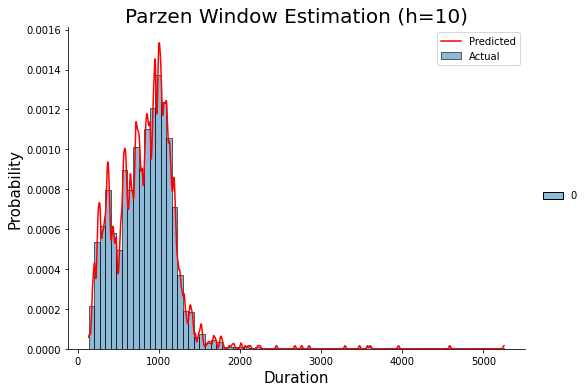
\includegraphics[scale=0.5]{q8/Q8_a.png}
    \caption{توزیع تخمین زده شده با $k = 10$}
    \label{fig:5}
    \end{center}
\end{figure}

\subsection*{ب}
مانند بخش الف این تمرین با تغییر هایپرپارامتر طبقه بند (همان طول پنجره) یادگیری و تخمین توزیع را انجام می‌دهیم نتایج در شکل \ref{fig:6} نشان داده شده‌اند. اینکه با افزایش  $h_{n}$  تابع توزیع پیش بینی شده نرم‌تر می‌شود کاملاً مشخص است.
\begin{figure}[h]
    \centering
    \subfigure[$h_{n} = 5$]{
    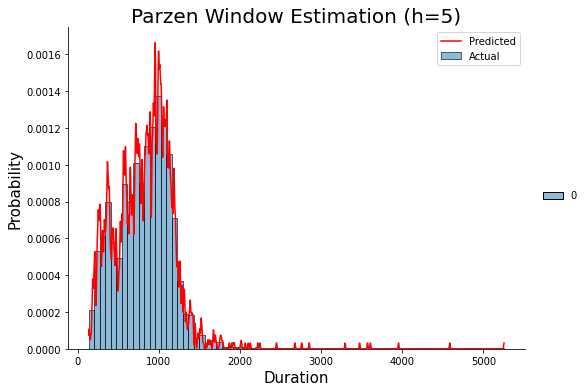
\includegraphics[width=.48\textwidth]{q8/Q8_b1.png}
    }
    \subfigure[$h_{n} = 25$]{
    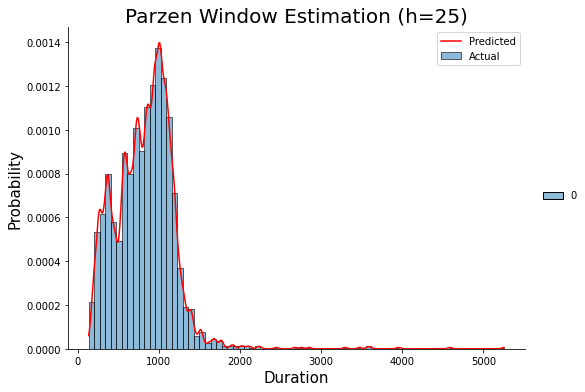
\includegraphics[width=.48\textwidth]{q8/Q8_b2.png}
    }
    \subfigure[$h_{n} = 125$]{
    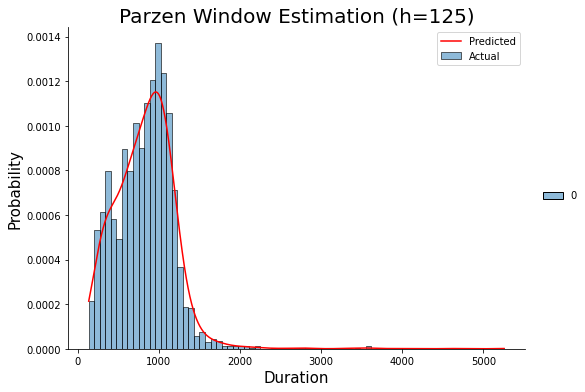
\includegraphics[width=.48\textwidth]{q8/Q8_b3.png}
    }
    \caption{توزیع‌های تخمین زده شده با طول پنجره متفاوت}
    \label{fig:6}
\end{figure}

\subsection*{ج}
در این قسمت داده‌ها را به طور تدریجی به تخمین‌زن می‌دهیم تا  روند تغییر و همگرا شدن به توزیع اصلی را ببینیم. این نمودار در شکل \ref{fig:7} آورده شده است.
\begin{figure}[h!]
    \begin{center}
    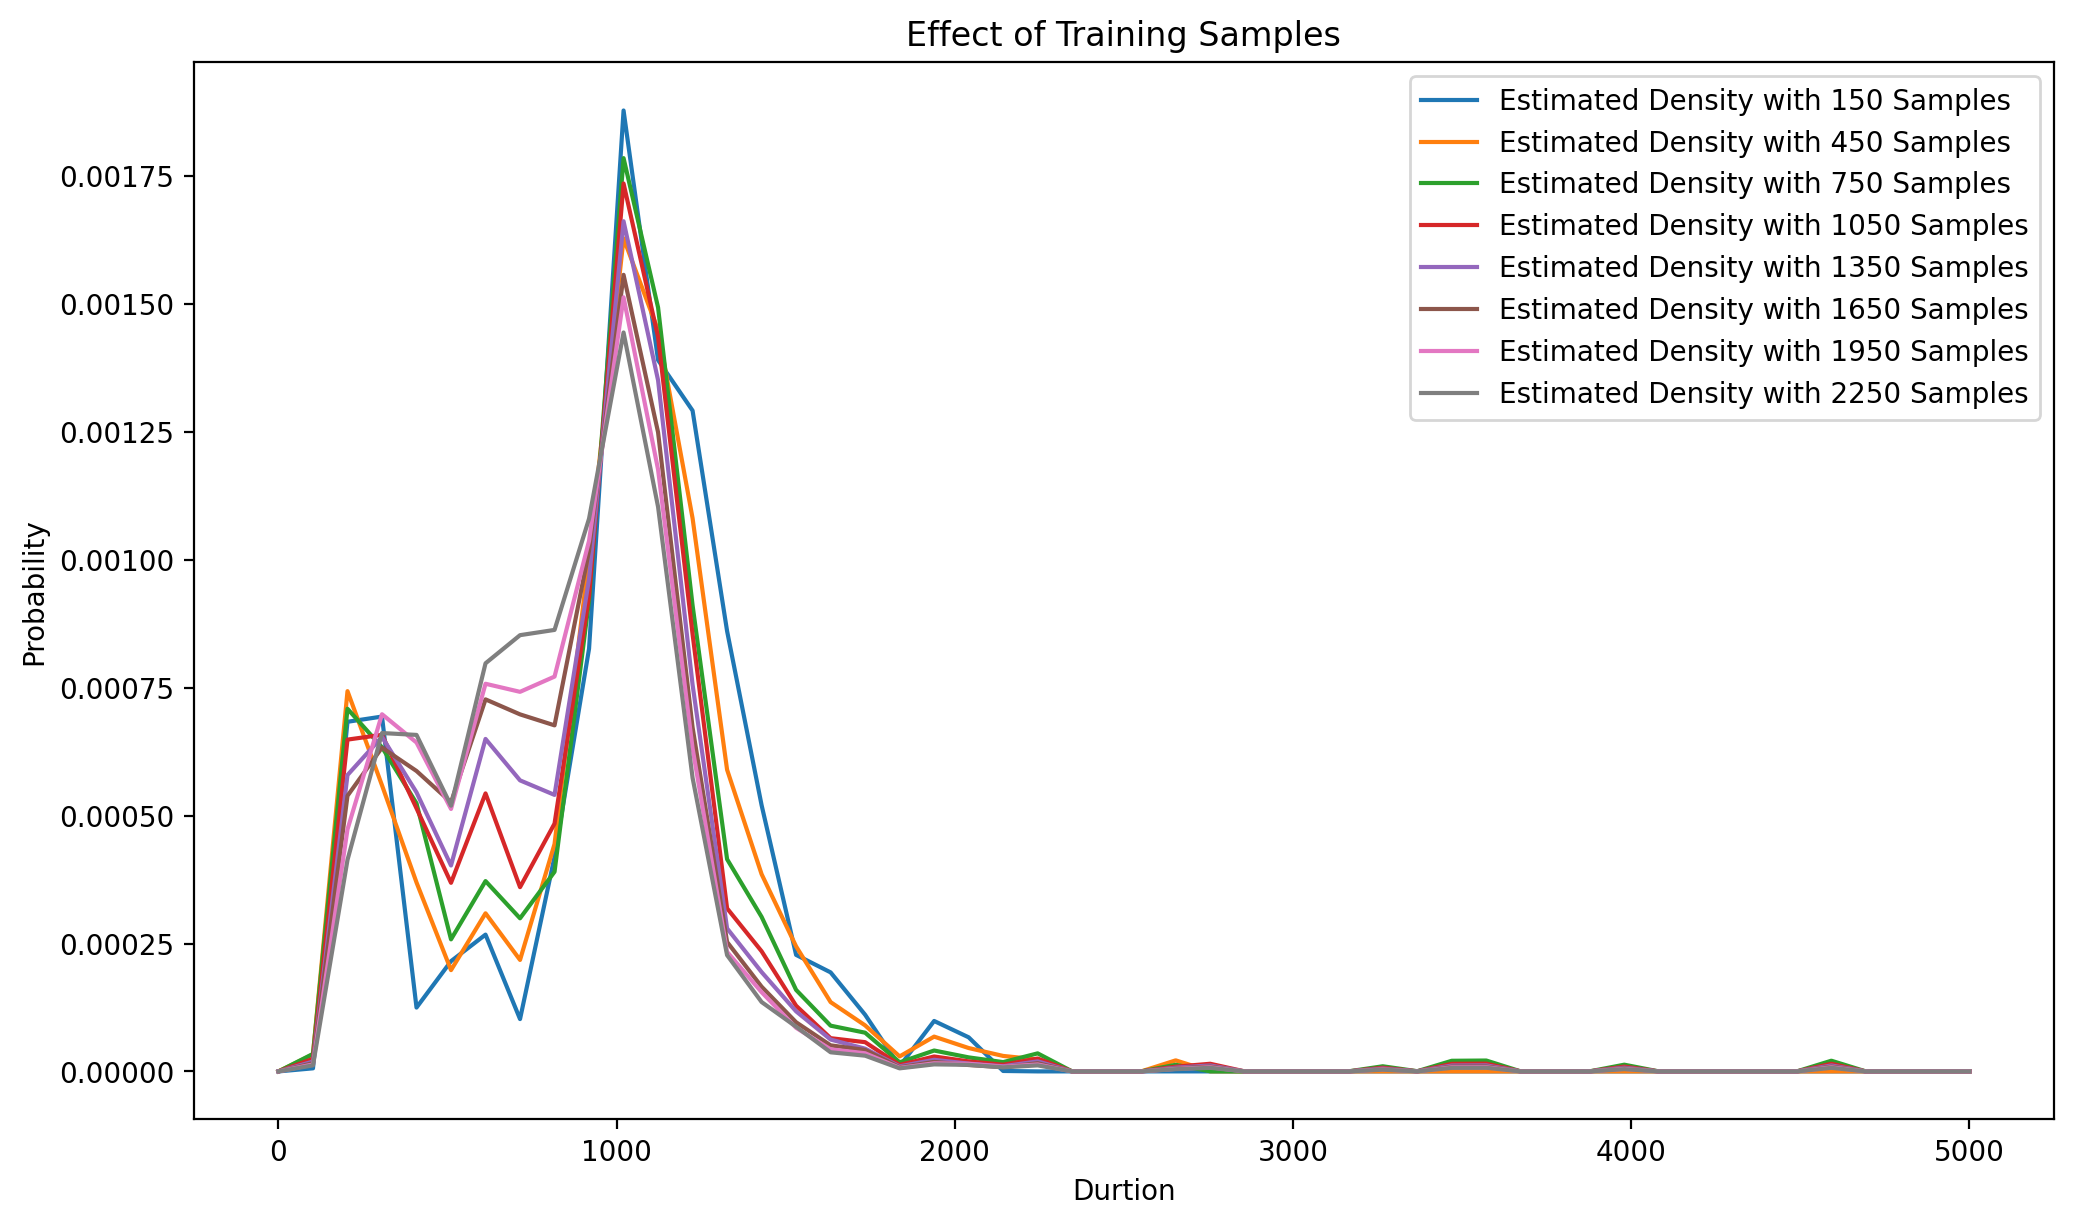
\includegraphics[scale=0.5]{q8/Q8_c.png}
    \caption{روند همگرایی تخمین نان‌پارامتری پنجره پارزن }
    \label{fig:7}
    \end{center}
\end{figure}

\subsection*{د}
در این قسمت با استفاده از \lr{KernelDensity} از کتابخانه \lr{scikit learn} نتایج قسمت الف را صحت سنجی می‌کنیم. \\
یک آبجکت \lr{KernelDensity} ساخته و طول پنجره را در آرگومان ورودی (\lr{band width}) تنظیم می‌کنیم. سپس داده‌های یادگیری را با فراخوانی تابع \lr{fit} به مدل می‌دهیم. در نهایت می‌توان با تابع \lr{score samples} احتمال داده‌های تست را حساب کرد. این تابع لگاریتم طبیعی احتمال را در خروجی باز می‌گرداند، پس لازم است آن‌ها را با تابع \lr{exp} از کتابخانه \lr{numpy} به احتمال تبدیل کرد.

\begin{figure}[h!]
    \begin{center}
    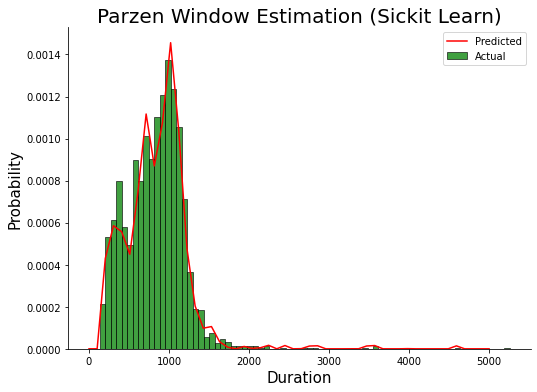
\includegraphics[scale=0.5]{q8/Q8_d.png}
    \caption{تخمین نان‌پارامتری پارزن با استفاده از کتابخانه \lr{scikit learn}}
    \label{fig:8}
    \end{center}
\end{figure}

\end{document}